\documentclass{article}

\usepackage{graphicx}
\usepackage{physics}
\usepackage{subcaption}
\usepackage{hyperref}
\usepackage{float}

\usepackage[left=2.5cm, right=2.5cm, top=2cm, bottom=2cm]{geometry}
\setlength{\parindent}{0em}
\setlength{\parskip}{0.8em}

\usepackage{caption}
\captionsetup{width=.9\textwidth}

\usepackage{biblatex}
\addbibresource{report.bib}

\title{Exam, TFY4235 Computational physics}
\author{Number}
\vspace{-8ex}
\date{}


\begin{document}
    \maketitle
    \section*{Introduction}
    The COVID-19 pandemic have showed how important it is to be able to simulate the spread of an infection throughout a population, and how much our behavior and travel patterns might change how this happens.
    SIR (Susceptible, Infected and Recovered), and the more advanced SEIIaR (Exposed, Infected asymptomatic), are mathematical models that aim to capture how pandemics spread throughout a simulation.
    They are vastly simplified and leave out a lot of the complications of a real world pandemic, but they still might give some lessons for what happens in the real world.
    This paper documents the implementation and results of the simulation of these models in Python, as described in \cite{exam}.
    It presents the result from different models, investigates how they respond to changing parameters and what the error due to numerical approximations or randomness inherit in the model.

    \section*{Implementation and Theory}
    All the different models used in this text follow the same basic form. 
    The goal is to find $x(t)$, given initial conditions $x(t_0)$, and a equation of the form
    \begin{equation*}
        f(x(t); \mathrm{args}) = \dv{x(t)}{t}.
    \end{equation*}
    In the first part, $x = (S, I, R)$, while later $x = (S_{ij}, E_{ij}, I_{ij}, Ia_{ij}, R_{ij})$ where $(ij)$ are different population groups. 
    This is accomplished using function \verb|integrate| in \verb|utilities.py|. 
    It takes as arguments the initial conditions \verb|x0|, the functions \verb|f| and \verb|step|, the list \verb|args| as well as the time step \verb|dt| and total time \verb|T| to simulate. 
    It then creates a discrete approximation of $x(t)$ by taking time steps given by the function \verb|step|. 
    \verb|step| is the particular \emph{scheme} used, for example Runge-Kutta 4, while \verb|f| defines the system. In the last model in this report, $356\times356\times5\times1800=1\,140\,624\,000$ floating point numbers are generated for each run of the simulation, which may result in the computer running out of RAM.
    However, event though a timestep of $\Delta t = 0.1$ is necessary to get accurate results, it is not necessary to store all time points.
    \verb|integrate| therefore takes the argument \verb|save|, which is the number of data points to store.
    The loop within \verb|integrate| has a inner loop which takes \verb|skip = (Nt-1)//(save-1)| time steps storing the value.
    
    In the SEIIaR commuter model, each step is calculated by drawing a random number, using a binomial or multinomial distribution, from each variable in the simulation.
    That means five random numbers for each cell in the population matrix.
    This is done in the function \verb|SEIIaR_commute| in \verb|utilities.py|
    This is being done using NumPy's binomial and multinomial functions, which supports bein given a array of populations to draw from.
    \footnote{The binomial distribution also supports that the probabilities are arrays, such that each popluation has a different probability.
    This is necessesary when calculating how many change from Susceptible to Exposed, as the probability for this depends on location.
    The multinomial function does \emph{not} support this, but it is luckily not needed here.}
    When drawing these random numbers, a lot of the populations that are drawn from are zero, as can be seen i \autoref{pop structure}.
    An effor to speed was therefore made by masking the arrays, such that only non-zero populations were left.
    This, however, did not change the running time of the simulation notacibly, as can be seen in \verb|profile.ipynb|.
    The second to lowest and lowest cells shows a profile of the simulation without and with the masking, and both the running time and the time of each line is nearly unchaged.
    This suggests that either the binomial/multinomial functions do not respect the masking, or that they simply are optimized for popluations of zero already.


    The equations that give the asymptotic behavior are both of the type $x = f(x)$, and can thus be approximated by recursion, given that they converge. 
    For $\mathcal{R}_0$ close to one, they converge increasingly slowly, and the program may reach maximum recursion depth. 
    For the parameters in this exercise, however, this was not a problem.

    When evaluating the precision of the different simulation schemes, a measure of error is needed.
    In this text, the measure of error for a simulation with time step $\Delta t_i$ is
    \begin{equation*}
        \Delta R_i = \frac{|R_i(t_0) - R_{\mathrm{ref}}(t_0)|}{R_{\mathrm{ref}}(t_0)},
    \end{equation*}
    where $R_{\mathrm{ref}}$ is some reference value of $R$ (Recovered) obtained by a simulation with a short step length, and $R_i$ is the value from the simulation with step length $\Delta t_i$.
    The difference is taken at some time $t_0$, which is chosen so that $t_0/\Delta t_i$ is an integer for the time steps in question.
    This is done such that several time steps may be compared with the same reference.
    Given a set of measurments $\{x_i\}_{i=1}^n$, the estimator for the mean and variance of the underlying distribution is 
    \begin{equation*}
        \mu = \frac{1}{n}\sum_{i=1}^n x_i, \quad s^2 = \frac{1}{n-1} \sum_{i=1}^n (x_i - \mu)^2.
    \end{equation*}
    $s$ is then not a measure of the error of the estimate of $\mu$, but rather a estimation of a parameter of the underlying distribution.
    How far from the mean can one expect a new observation $x_{n+1}$ to be.
    The standard error, $\sigma = \sqrt{s^2/n}$, gives a estimation of the standard deviation of the sampling distribution, and is therefore used as a measure of the error in this text.\footnote{\url{https://en.wikipedia.org/wiki/Standard_error}} 
    \section*{Results}
    \subsection*{Deterministic SIR model}
    The first model is the deterministic SIR model, given by a set of coupled ODEs \cite{exam}. 
    In this text, the Runge-Kutta 4 scheme was used, as it is both a simple yet precise scheme.
    \autoref{SIR} demonstrates that $S$ and $R$ approaches the expected asymptotes, and that $I$ grows exponentially in the beginning at the rate expected.
    \autoref{conv det} shows an error estimation of different integration schemes.
    The error is found by comparing to a solution found by using the RK4-solver, and $\Delta t = 0.01$.
    This illustrates why the choice of $\Delta t = 0.1$ is sufficient, as numerical errors start playing a large role for larger $\Delta t$.
    
    Adjusting the $\beta$-parameter will affect how fast the virus spreads, thus ``flattening the curve'', as illustrated in \autoref{flattening}.
    This shows that the highest $\beta$ that ensures the maximum fraction of population   at once below $20\%$ is $\beta=0.228$. 
    \autoref{vax} shows the fraction of the population must be vaccinated \emph{before} the outbreak to stop exponential growth. 
    At the start of the simulation, the number of infected grows exponentially, i.e. $I \propto \exp(\alpha t)$ for some $\alpha$.
    A partially vaccinated population can be modeled by setting $R(0)$ equal the proportion of the population that is vaccinated.
    The result shows that $60\%$ or more must be vaccinated to avoid exponential growth, i.e. $\alpha\leq 0$. 
    These results could be made more precise by extrapolation, more simulation or searching with the bisection method, but the crudeness of the model means higher precision is wasted.

    \begin{figure}[H]
        \centering
        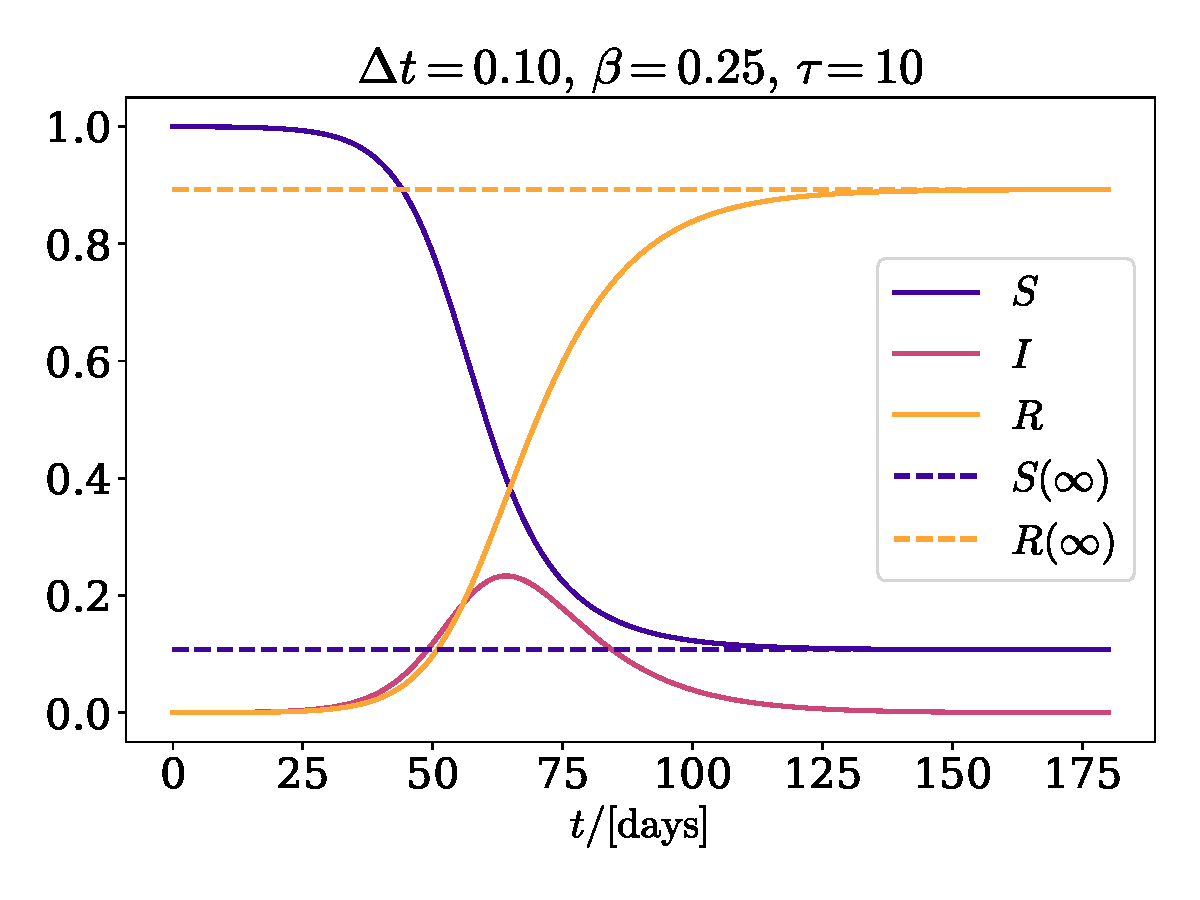
\includegraphics[width=.49\textwidth]{../plots/2A/TestSIR}
        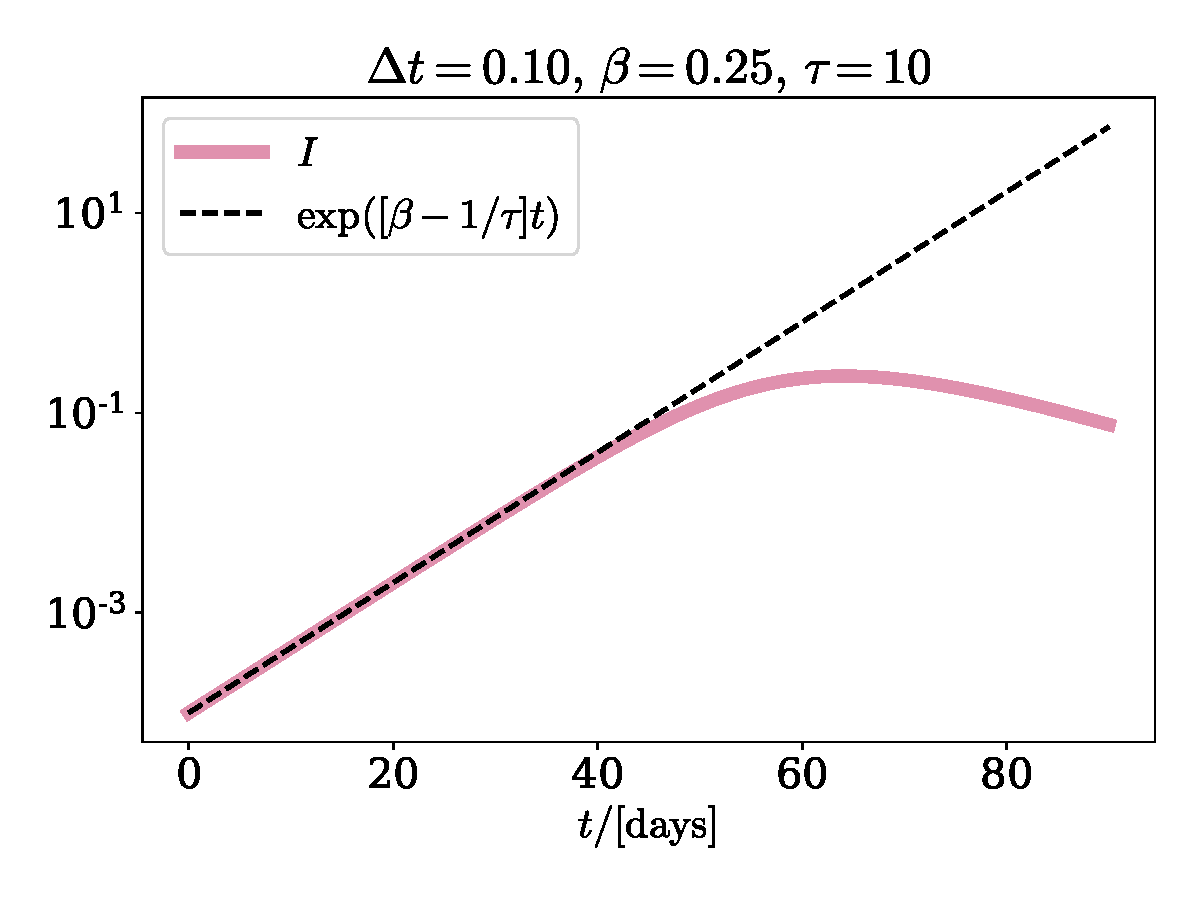
\includegraphics[width=.49\textwidth]{../plots/2A/TestI}
        \caption{On the left, the fraction of the population that is in each group, over time.
        The plot on the right shows how the infection spreads exponentially in the begining}
        \label{SIR}
    \end{figure}

    \begin{figure}[H]
        \centering
        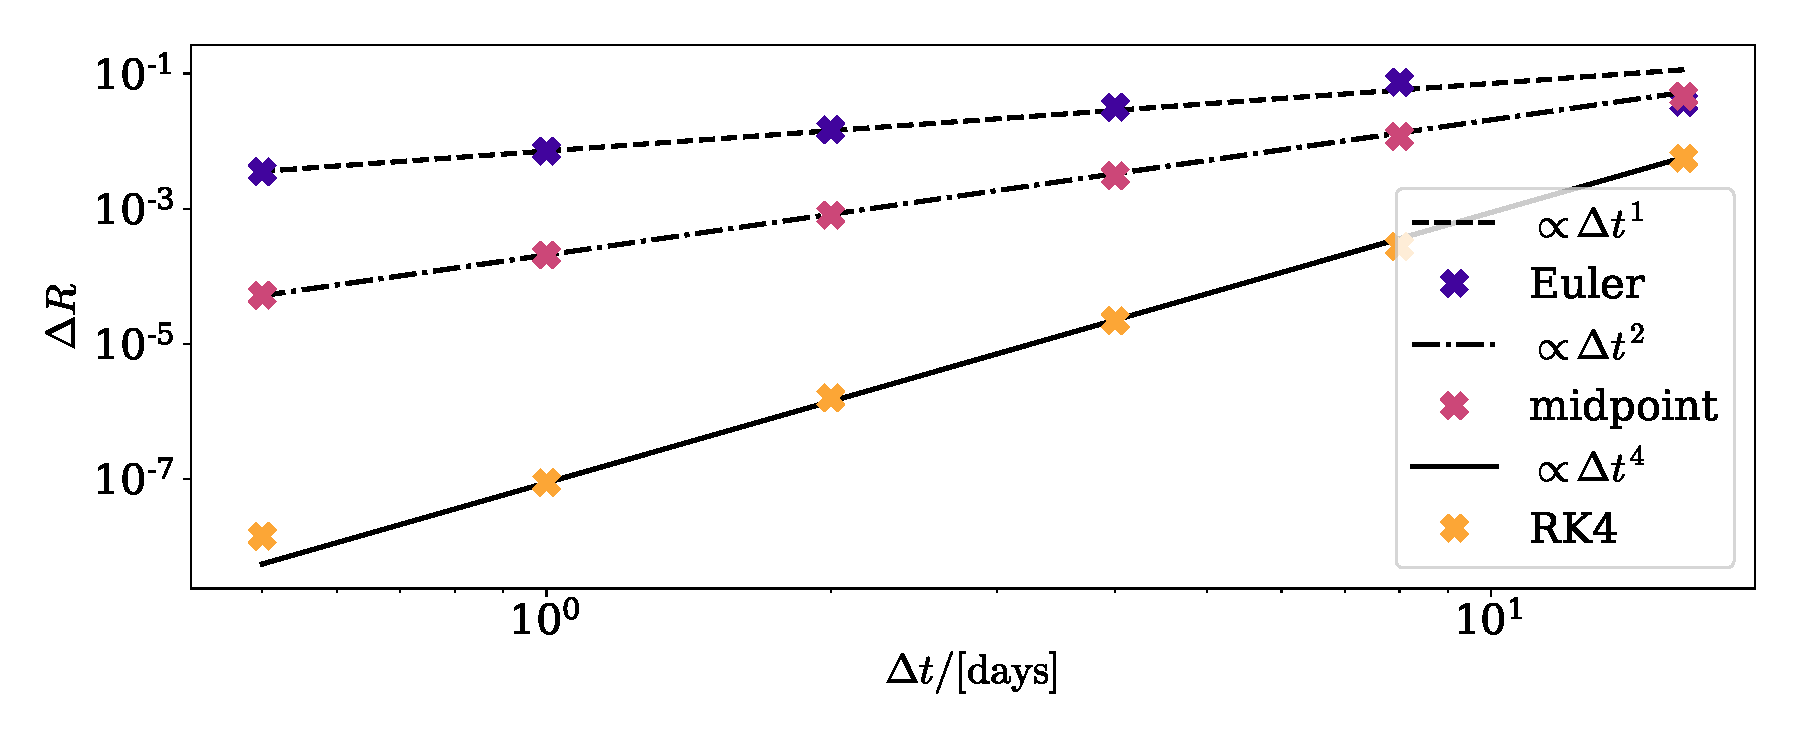
\includegraphics[width=.6\textwidth]{../plots/2A/conv}
        \caption{The error, after, 128 days, of different integration schemes.
        All are compared with RK4, with steplength $\Delta t = 0.01$.}
        \label{conv det}
    \end{figure}

    \begin{figure}[H]
        \centering
        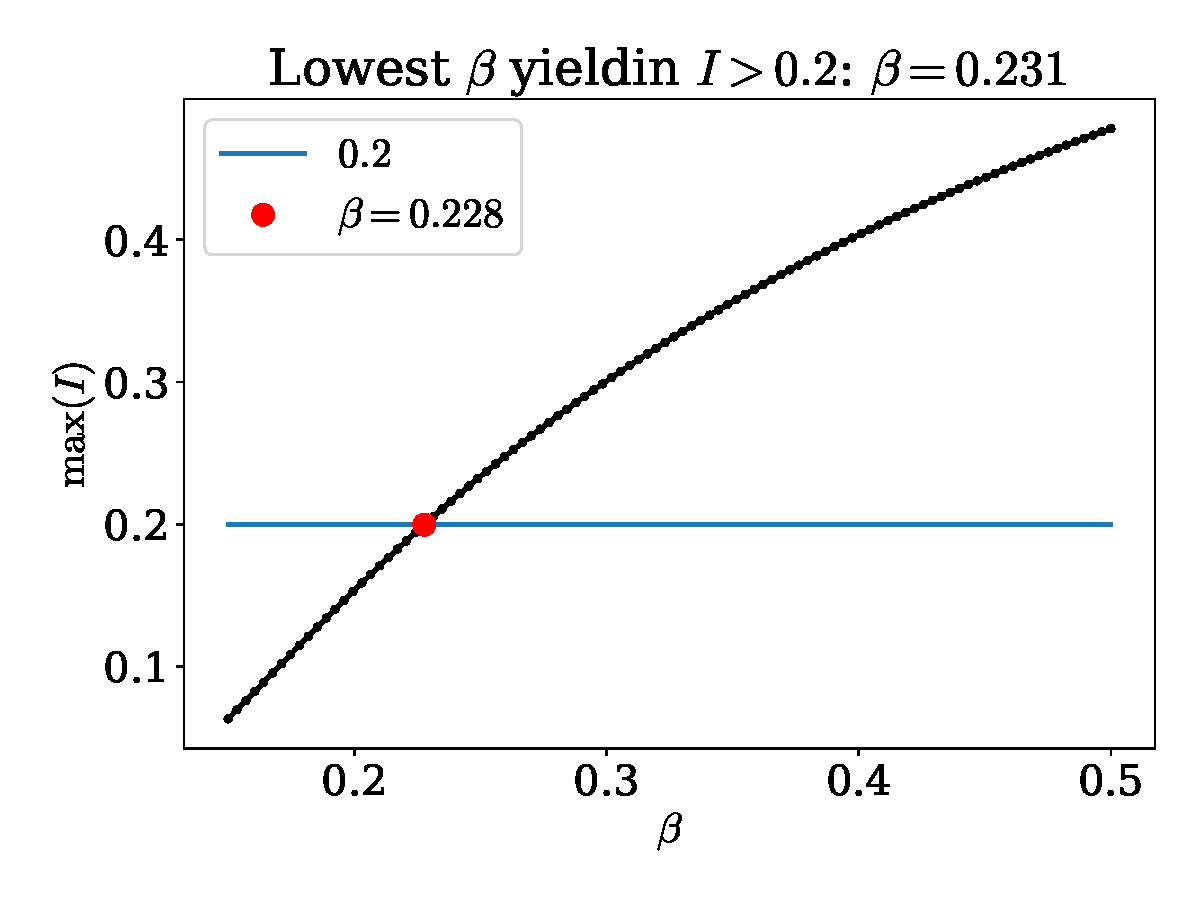
\includegraphics[width=.49\textwidth]{../plots/2A/flatten.pdf}
        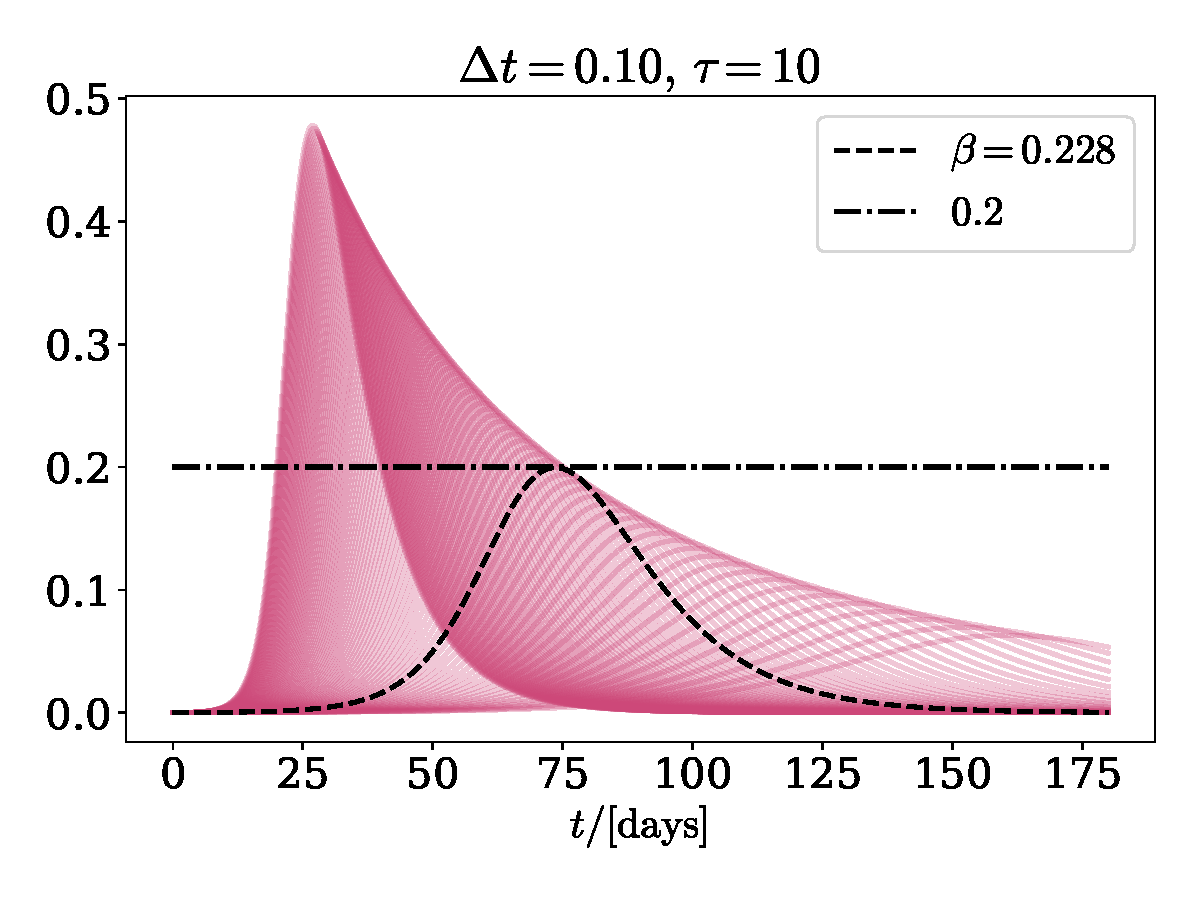
\includegraphics[width=.49\textwidth]{../plots/2A/flattenIs.pdf}
        \caption{The figure on th eright shows the maximum fraction of infected, as a function of $\beta$. 
        The largest value of $\beta$ such that the maximum is beneath $0.2$ is indicated. 
        On the right, the corresponding infection curves.}
        \label{flattening}
    \end{figure}

    \begin{figure}[H]
        \centering
        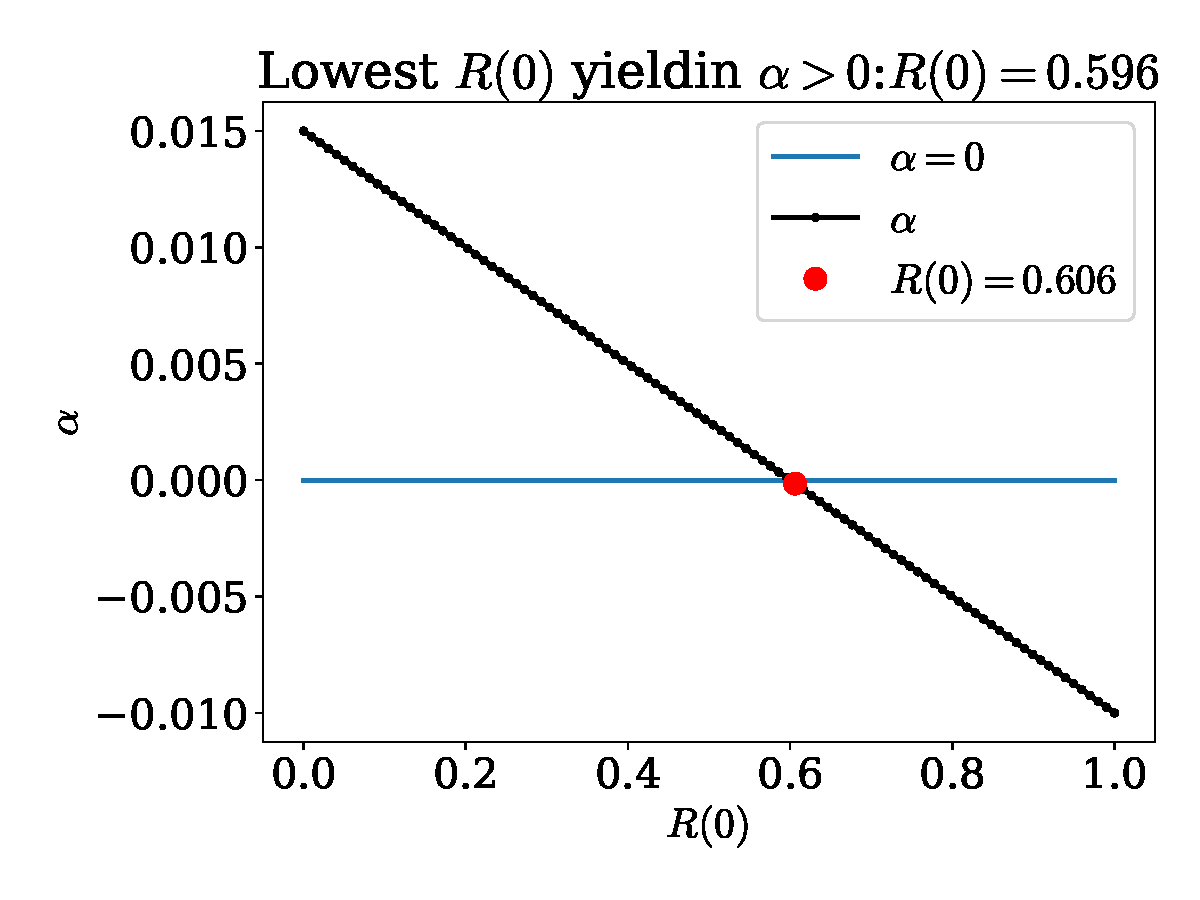
\includegraphics[width=.49\textwidth]{../plots/2A/vax.pdf}
        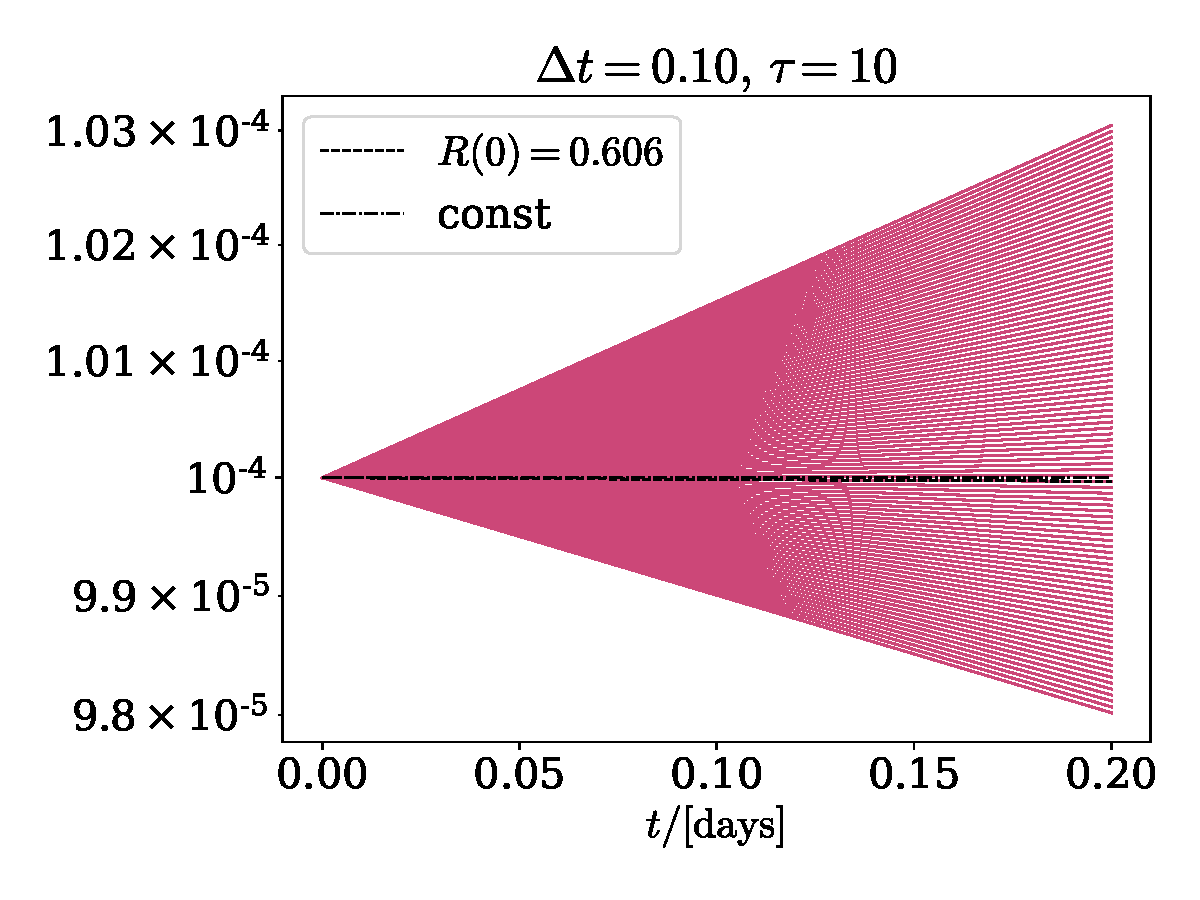
\includegraphics[width=.49\textwidth]{../plots/2A/vax_R.pdf}
        \caption{The plot on the left shows minimum $R(0)$, i.e. fraction of vaccinated, that prevents exponential growth.
        On the right, a log-plot of the growht of infected at the very begining.}
        \label{vax}
    \end{figure}

    \subsection*{Stochastic SIR model}
    Next, the stochastic version of SIR model is simulated. \autoref{stochastic SIR} shows the result of 100 runs, which all give result close to that of the deterministic one. 
    All simulation uses a population of 100\,000, but the plots are normalized such that all variables are proportions of the total poplation.
    Due to the stochastic nature of the simulation, there is a difference in exactly when the exponential growth starts. 
    however, as the figure on the right shows, when it does, it grows exponentially at the same rate as the deterministic model. 
    This is also the reason for the spread of the runs around the dashed line in the figure on the right.
    The early days of the infection is susceptible to fluctuations.
    We also see the stochastic model tend to be later than the deterministic.
    These used step length $\Delta t = 0.1$ for the stochastic model. 
    \autoref{conv} is a plots the relative error of the simulation $\Delta R$, as discussed in the Theory section.
    The values are obtained by taking an average of 100 runs for each value of $\Delta t$.
    This result justifies the use of $\Delta t = 0.1$, as it leads to quick simulations, while resulting in errors around $0.2\%$
    Furthermore, the results imply that the method converges as $\Delta t^1$, which means that large gains in precision will be costly.
    
    The stochastic nature of this model makes it possible for the infection to die out, even with $\mathcal{R}_0>1$, by pure chance. 
    \autoref{Disappear} shows a probability for the infection terminating without spreading through the population, for different number of initially infected $I(0)$.
    This data is obtained by running the simulation 1\,000 times for each initial condition, and terminating when it either reach 100 or 0 infected.
    100 infected is observed to yield very high probability of the disease spreading exponentially, and is thus used as a proxy for this.
    This assumption is backed up by the result shown in the figure, where the probability for the infection stopping early is negligible already at $I=10$. 
    $I=0$ means that the infection will no longer spread, and if it does so without ever hitting $I=100$, then the outbreak has disappeared.
    Let $x_i\in\{0, 1\}$ be the outcome of simulation $i$, equalling 0 if the outbreaks dies out, 1 if it does not.
    The probability of the infection dying out is then a Bernoulli process, with a probability $p$ of dying out, which depends on how many are initially exposed.
    \autoref{Disappear} shows the estimation of the probability of the outbreak dying out, together with the standard error as described in the Theory section, from 1000 runs of the simulation for each initial number of infected.

    \begin{figure}[H]
        \centering
        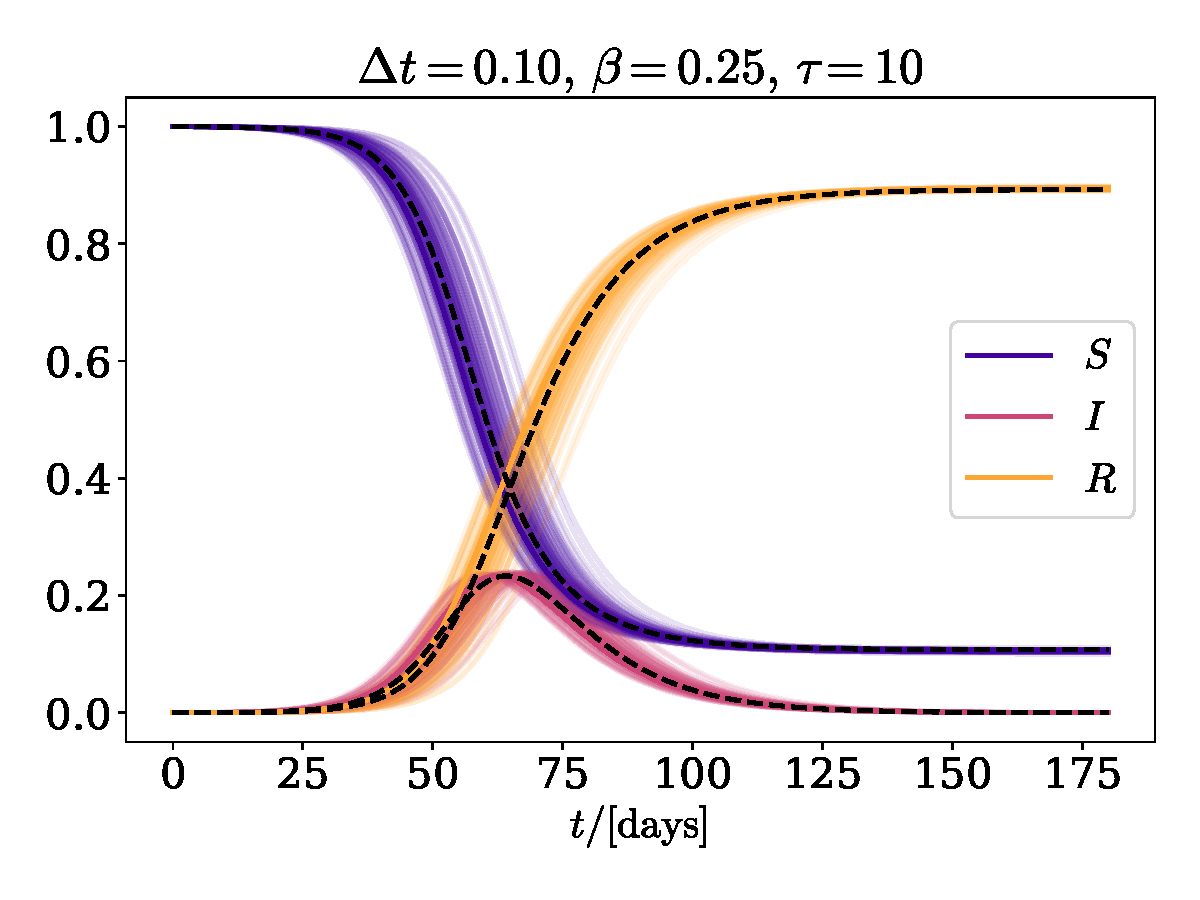
\includegraphics[width=.49\textwidth]{../plots/2B/TestSIR_stoch.pdf}
        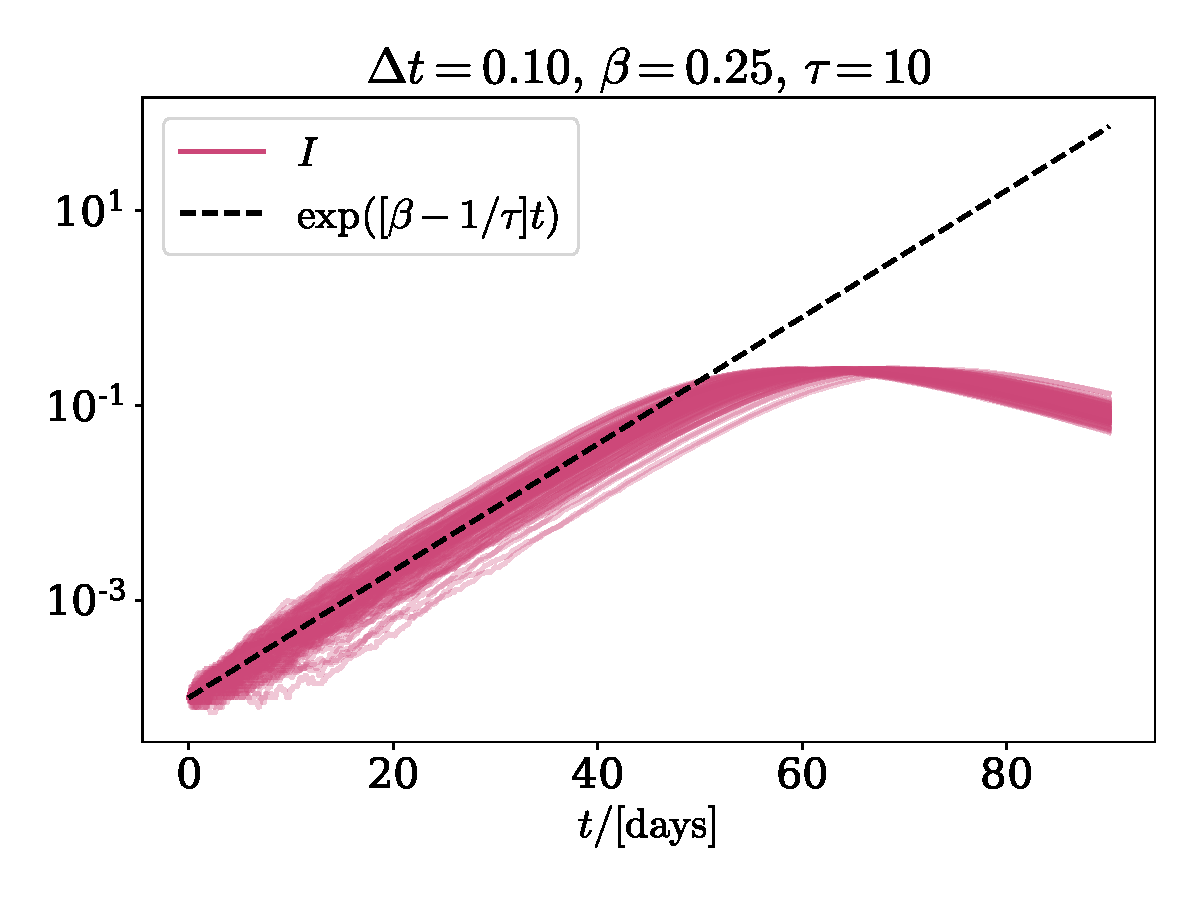
\includegraphics[width=.49\textwidth]{../plots/2B/TestI_stoch.pdf}
        \caption{100 runs of the stochastic SIR model. All runs are close to the deterministic, showed as dashed lines.}
        \label{stochastic SIR}
    \end{figure}

    \begin{figure}[H]
        \centering
        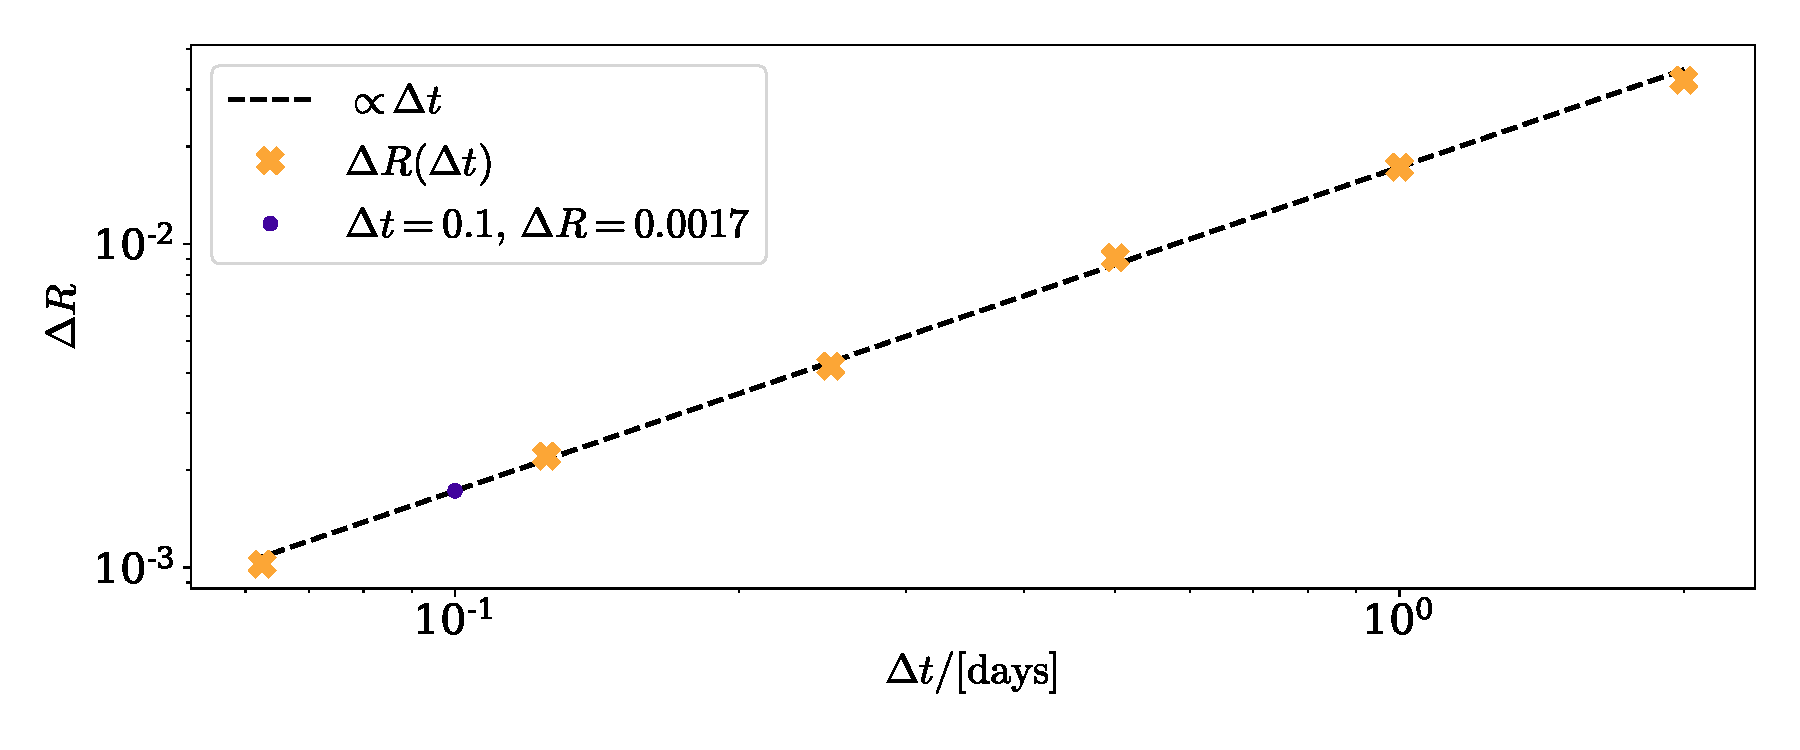
\includegraphics[width=.7\textwidth]{../plots/2B/conv.pdf}
        \caption{The relative eviation of the value of $R$ at $t_0=200 \, \mathrm{ days }$, for different step lengths $\Delta t$.}
        \label{conv}
    \end{figure}


    \begin{figure}[H]
        \centering
        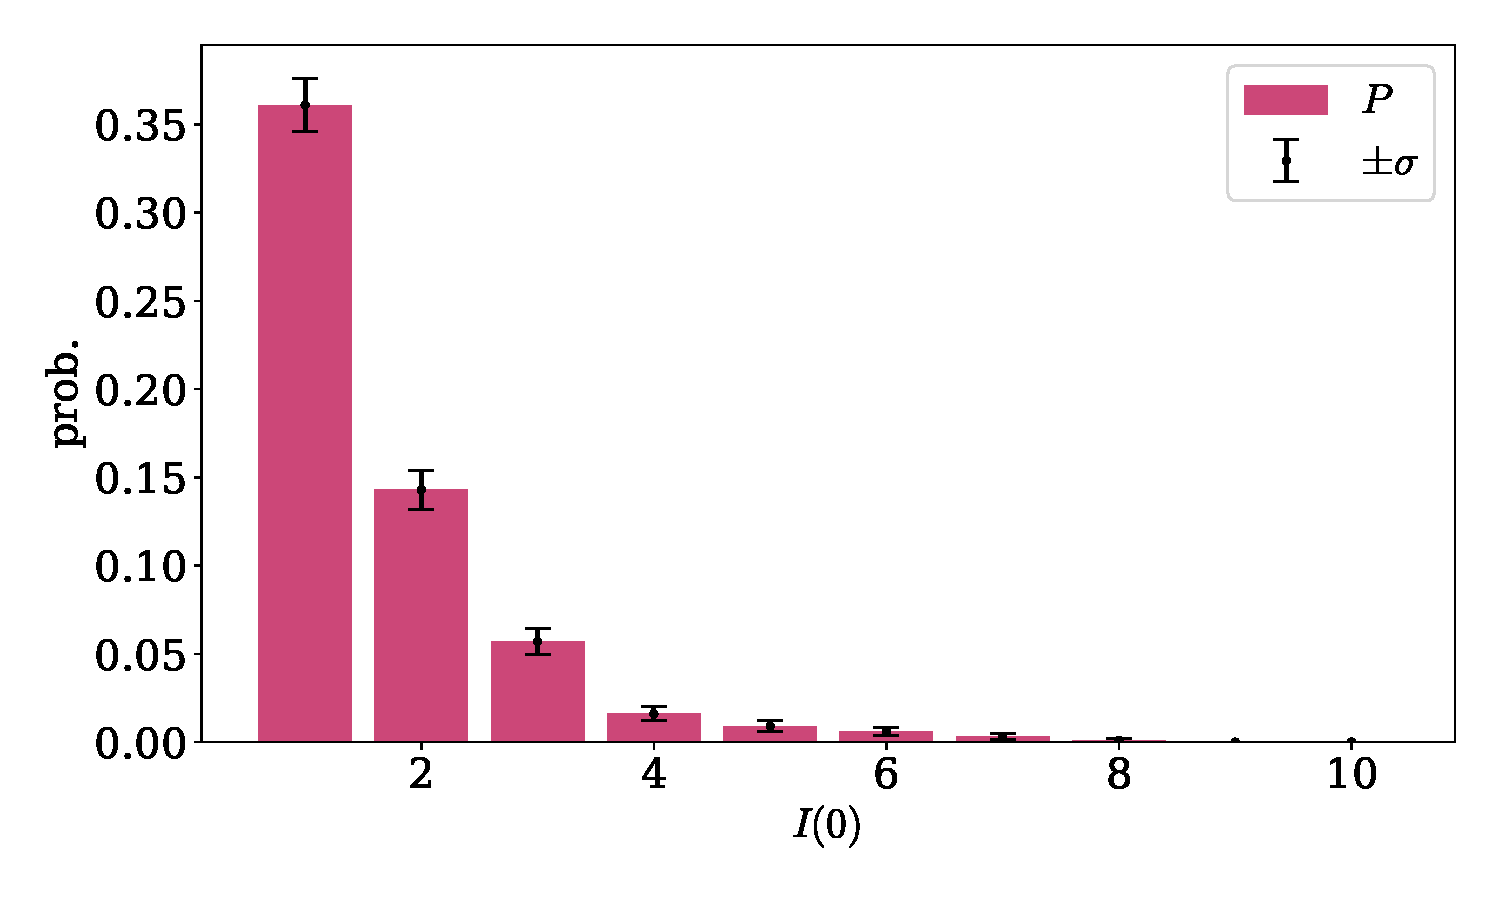
\includegraphics[width=.7\textwidth]{../plots/2B/disappear.pdf}
        \caption{The probability that the infection dies, for different starting values of $I$. Each probability is caculated from an average of 1\,000 runs, while the error bar indicate the standard error as described in the text.}
        \label{Disappear}
    \end{figure}

    \subsection*{SEIIaR model}
    The SEIIaR model incorporates the possibility of asymptomatic infection, $I_a$, and a incubation period, $E$ (Exposed), as well as a set of new parameters, described in \cite{exam}.
    From here on all parameters are as given in the exam \cite{exam}, except where otherwise is explicitly written.
    \autoref{SEIIaR} shows 10 runs of the simulation, and compares it to the result from the deterministic SIR model.
    The same asymptotic values are reach for $S$ and $R$, however, due to the incubation period, the raise in infection is delayed somewhat compared to both the stochastic and deterministic SIR models.
    As in the stochastic SIR model, there is a spread in just when the exponential growth begins, however all models have the same asymptomatic behavior.
    \autoref{SEIIaR conv} show a estimation of the error, where a simulations with different time step is compared to a reference simulation, all averaged over 100 runs.
    This shows that a timestep $\Delta t = 0.1$ should still yield high precision.

    Infected people with symptoms, $I$, can self isolate, and thus decrease the spread of the disease.
    This is controlled by the $r_a$ parameter.
    If it is $1$, the symptomatic are as likely to infect others as $\mathcal{R}_0 = \beta \tau $ would suggest. 
    However, if it is less due to for example isolation, then the spread might subside.
    \autoref{isolation} shows how $r_s$ affects the spread of the infection.
    \autoref{isolation1} illustrates the early evolution of the exposed population, $E$, for 101 values of $r_s\in [0, 1]$.
    Each line is an average of 100 runs.
    Due to the exposed population not being infectious, it will initially decrease.
    The measure of the exponential increase is therefore taken as $\alpha = \ln\left(E(20)/E(5)\right)/(15 \mathrm{days})$.
    If $\alpha>0$, then this is counted as exponential growth, and thus a outbreak.
    \autoref{isolation1} shows that \emph{the lowest $r_s$ that do not lead to an avereage exponential growth} is $r_s = 0.42$.
    \autoref{isolation2} shows a slightly different measure---the probability that a value for $r_s$ results in exponential growth---together with the estimated standard error.
    A point of comparison between the two measures is \emph{the higgest value of $r_s$ that gives a less than 50\% chance of exponential growth.}
    The highest measured value that fullfils this criterion is $r_s = 0.43$.
    It also shows the best fit to a Sigmoid curve, obtained using SciPy's \verb|optimize.curve_fit|.
    Altoug this function seem to describes the beahvior accuratly, there is no theoretical background for the choice.
    These two method yield slightly different results.
    \autoref{isolation1} shows how, on average, a outbreak wil evolve.
    However, due to the random nature of both the model and a real outbreak, each individual instatioation might turn out differently.
    \autoref{isolation2}, on the other hand, gives the probability that a given outbreak with a value for $r_s$ will yield exponential growth.
    This is therefore a better measure for evaluating single outbreaks where the parameters are known.

    \begin{figure}[H]
        \centering
        \begin{subfigure}{.49\textwidth}
            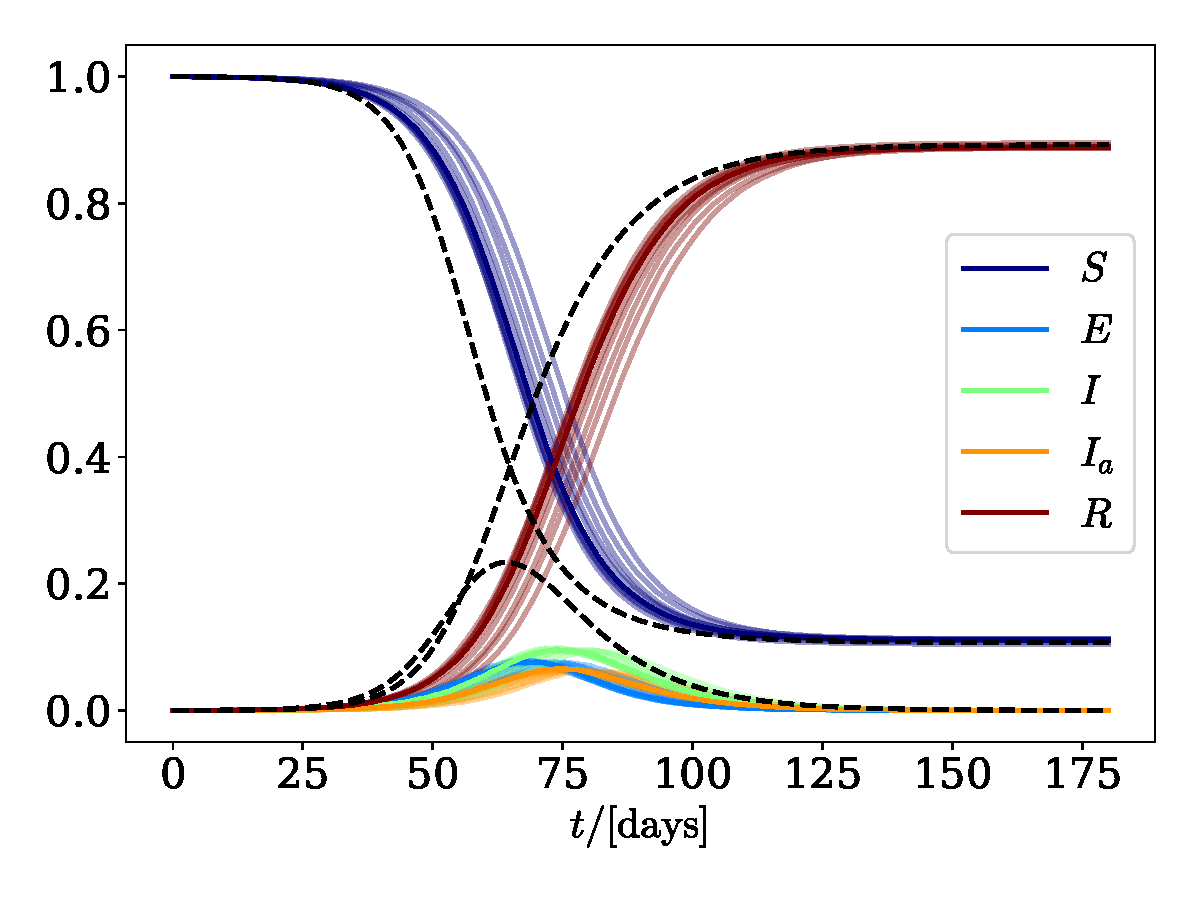
\includegraphics[width=\textwidth]{../plots/2C/TestSEIIaR.pdf}
            \caption{10 runs of the SEIIaR model.}
            \label{SEIIaR}
        \end{subfigure}
        \begin{subfigure}{.49\textwidth}
            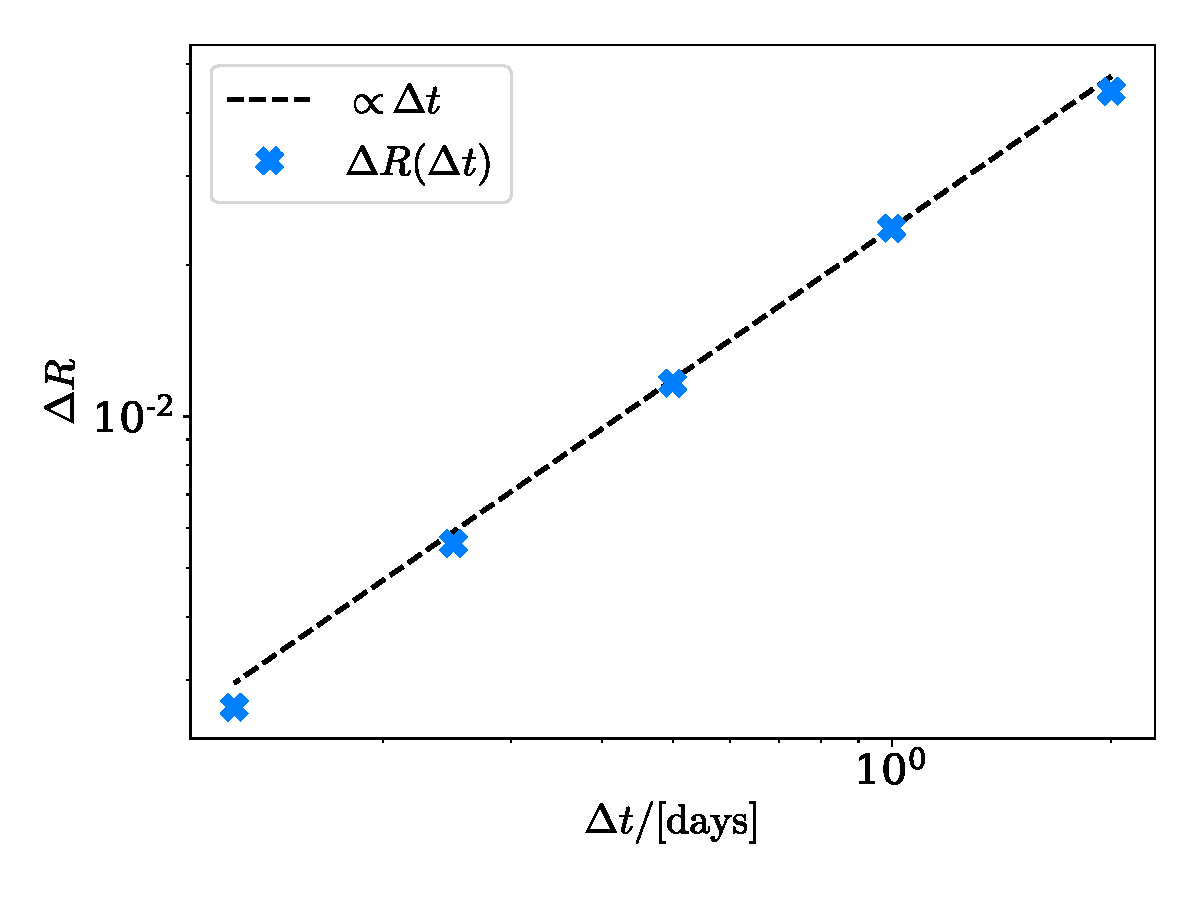
\includegraphics[width=\textwidth]{../plots/2C/conv.pdf}
            \caption{Error relative a reference run of the SEIIaR model.}
            \label{SEIIaR conv}
        \end{subfigure}
    \end{figure}

    \begin{figure}[H]
        \centering
        \begin{subfigure}{.49\textwidth}
            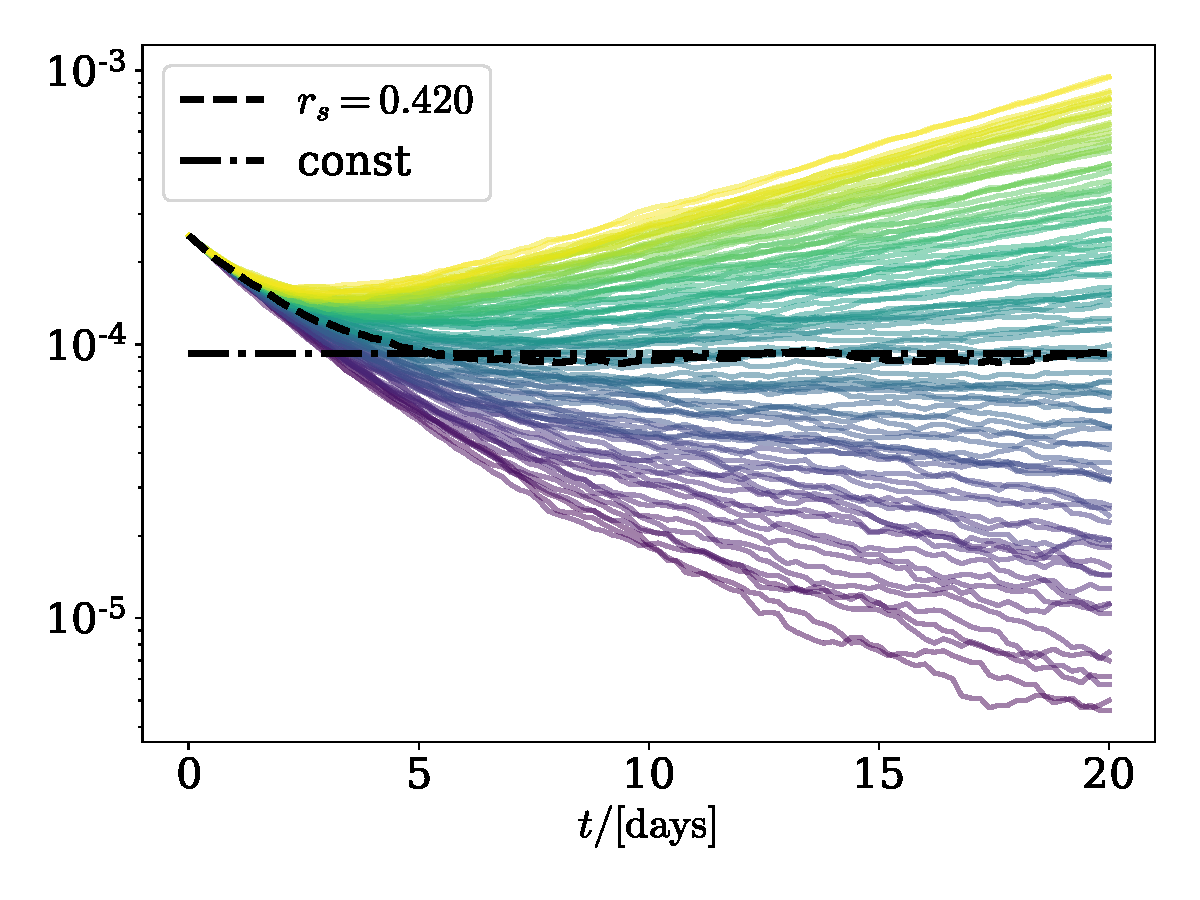
\includegraphics[width=\textwidth]{../plots/2C/isolation.pdf}
            \caption{The early evolution of the exposed (E) in the pandemic, for values of $r_s$ between 1 (top) an 0 (bottom).
             Each line is an average of 100 simulation runs.}
            \label{isolation1}
        \end{subfigure}
        \begin{subfigure}{.49\textwidth}
            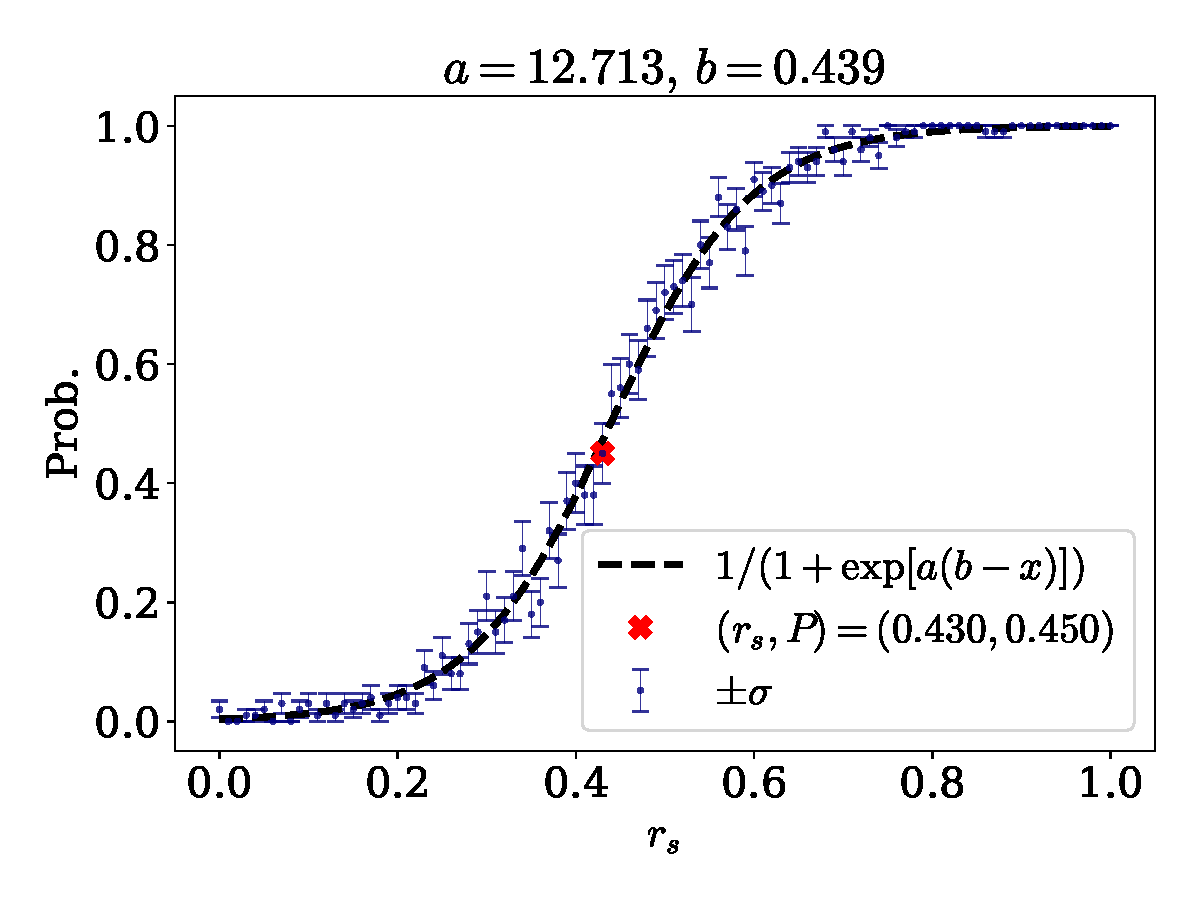
\includegraphics[width=\textwidth]{../plots/2C/isolation2_prob.pdf}
            \caption{The probability of exponential growth as a function of $r_s$, with the standard error indicated by errorbars.
            The cross indicates the higgest value of $r_s$, below 50\%.}
            \label{isolation2}
        \end{subfigure}
        \caption{Two different ways of measuring which value of $r_s$ gives exponential growth.}
        \label{isolation}
    \end{figure}


    \subsection*{SEIIaR commuter model}
    The last complication of the model is to include the fact that people live and work at different places, and might bring with them the infection when commuting. 
    The traveling pattern of the population is encoded in a matrix, as described in \cite{exam}.
    Given a matrix without off diagonal elements, each city should evolve exactly as they do in the non-commuter SEIIaR model.
    This is thus a good check on the implementation.
    \autoref{SEIIaR commute} shows the result in one of the cities of such a run.
    This is one of two towns, in a model without commuters, and a comparison with \autoref{SEIIaR} confirms that the results are the same.
    Furthermore, the error showed in \autoref{SEIIaR commute conv} behaves as the non-commuter model.
    Another test for the commuter model is to let the entire population be commuters, i.e. only off-diagonal elements are non zero, and start with infections only in one of these populations.
    Then, the spread should be contained to this population.
    This case is illustrated in \autoref{All commuters}, confirming that the model behaves as expected.

    This method is then used to simulate the system with 2 towns, described by the matrix in Equation 10 in \cite{exam}.
    The result from an average of then runs is showed in \autoref{two towns}, where each variable is plotted for each town.
    The peak of the infection is reached day 56 in town 1, while it is not before day 91 in Town 2.
    The total fraction of both towns that eventually gets the infection, however, is almost exactly the same, as the parameters are the same.
    Next, a system with 10 towns is simulated. 
    In this system, there are two large towns, town 1 and 5, and eight smaller towns, in groups of four which are connected to one of of the large towns.
    \autoref{nine towns} shows the evolution of the infection.
    The infection starts in town 2, which explains why it is the first to reach the peak of the infection, at day 57.
    It then spreads to town 1, as it is a hub connected to town 2, which has the peak of its infection at day 103. 
    Town 3, 4 and 4, all satellites of town 1 all hit their peak around day 120.
    The infection then spreads to the other hub, town 6, as it is connected to town 1.
    Its peak is at day 145, before it at last spreads to the satellites of town 6, town 7, 8, 9 and 10, which all have their peak around day 160.

    \begin{figure}[H]
        \centering
        \begin{subfigure}{.49\textwidth}
            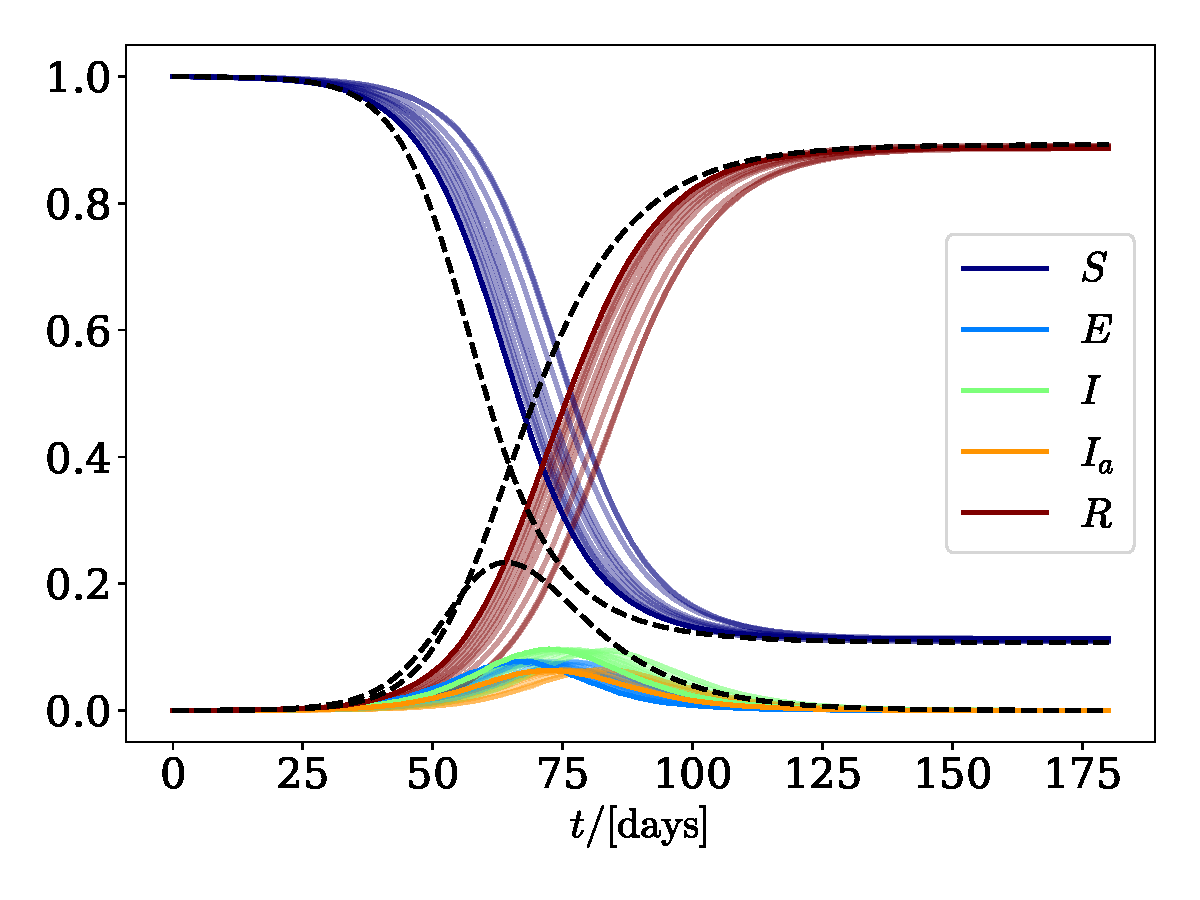
\includegraphics[width=\textwidth]{../plots/2D/TestSEIIaR_commute.pdf}
            \caption{results in town 1 of 10 runs of the SEIIaR commuter model, where all off diagonal elements are zero.}
            \label{SEIIaR commute}
        \end{subfigure}
        \begin{subfigure}{.49\textwidth}
            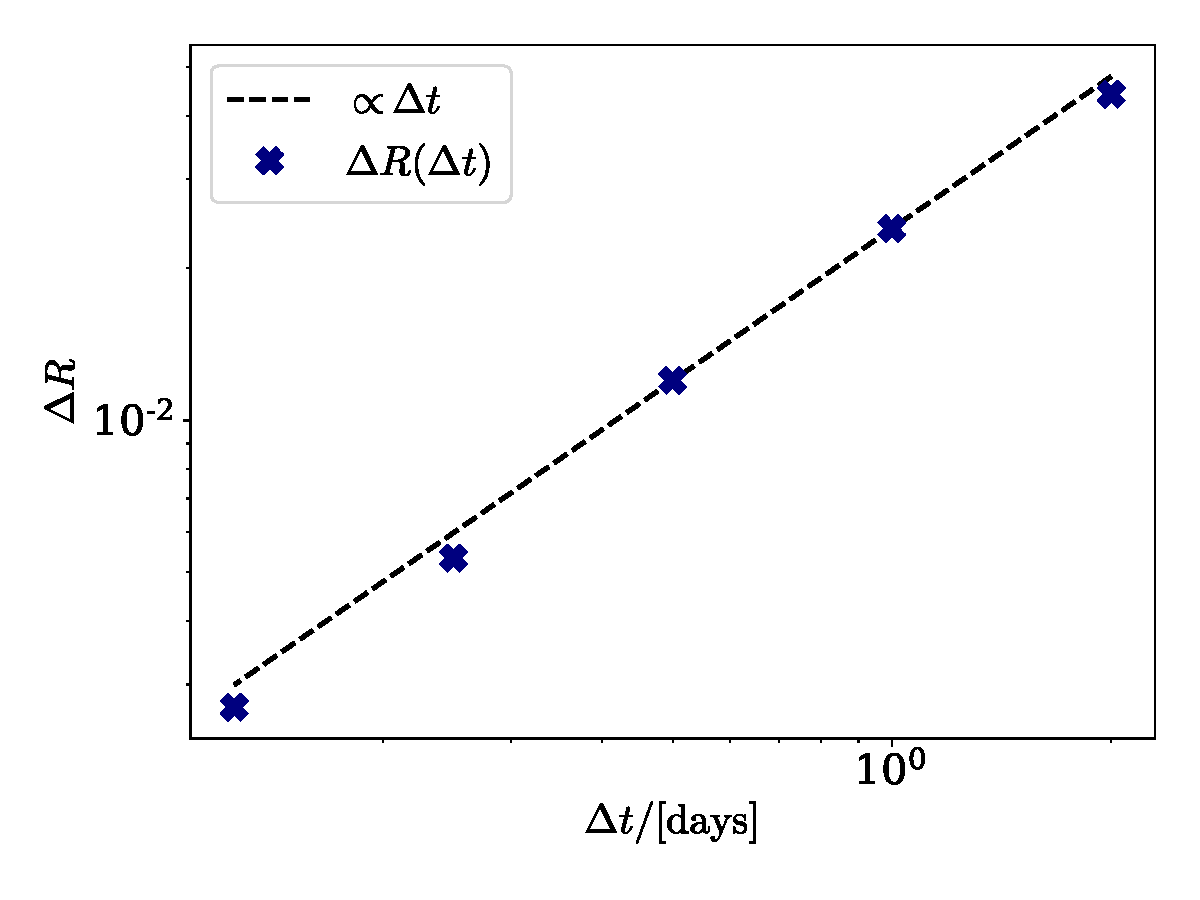
\includegraphics[width=\textwidth]{../plots/2D/conv.pdf}
            \caption{The error as a function of steplength in the same system as (a).}
            \label{SEIIaR commute conv}
        \end{subfigure}
    \end{figure}

    \begin{figure}[H]
        \centering
        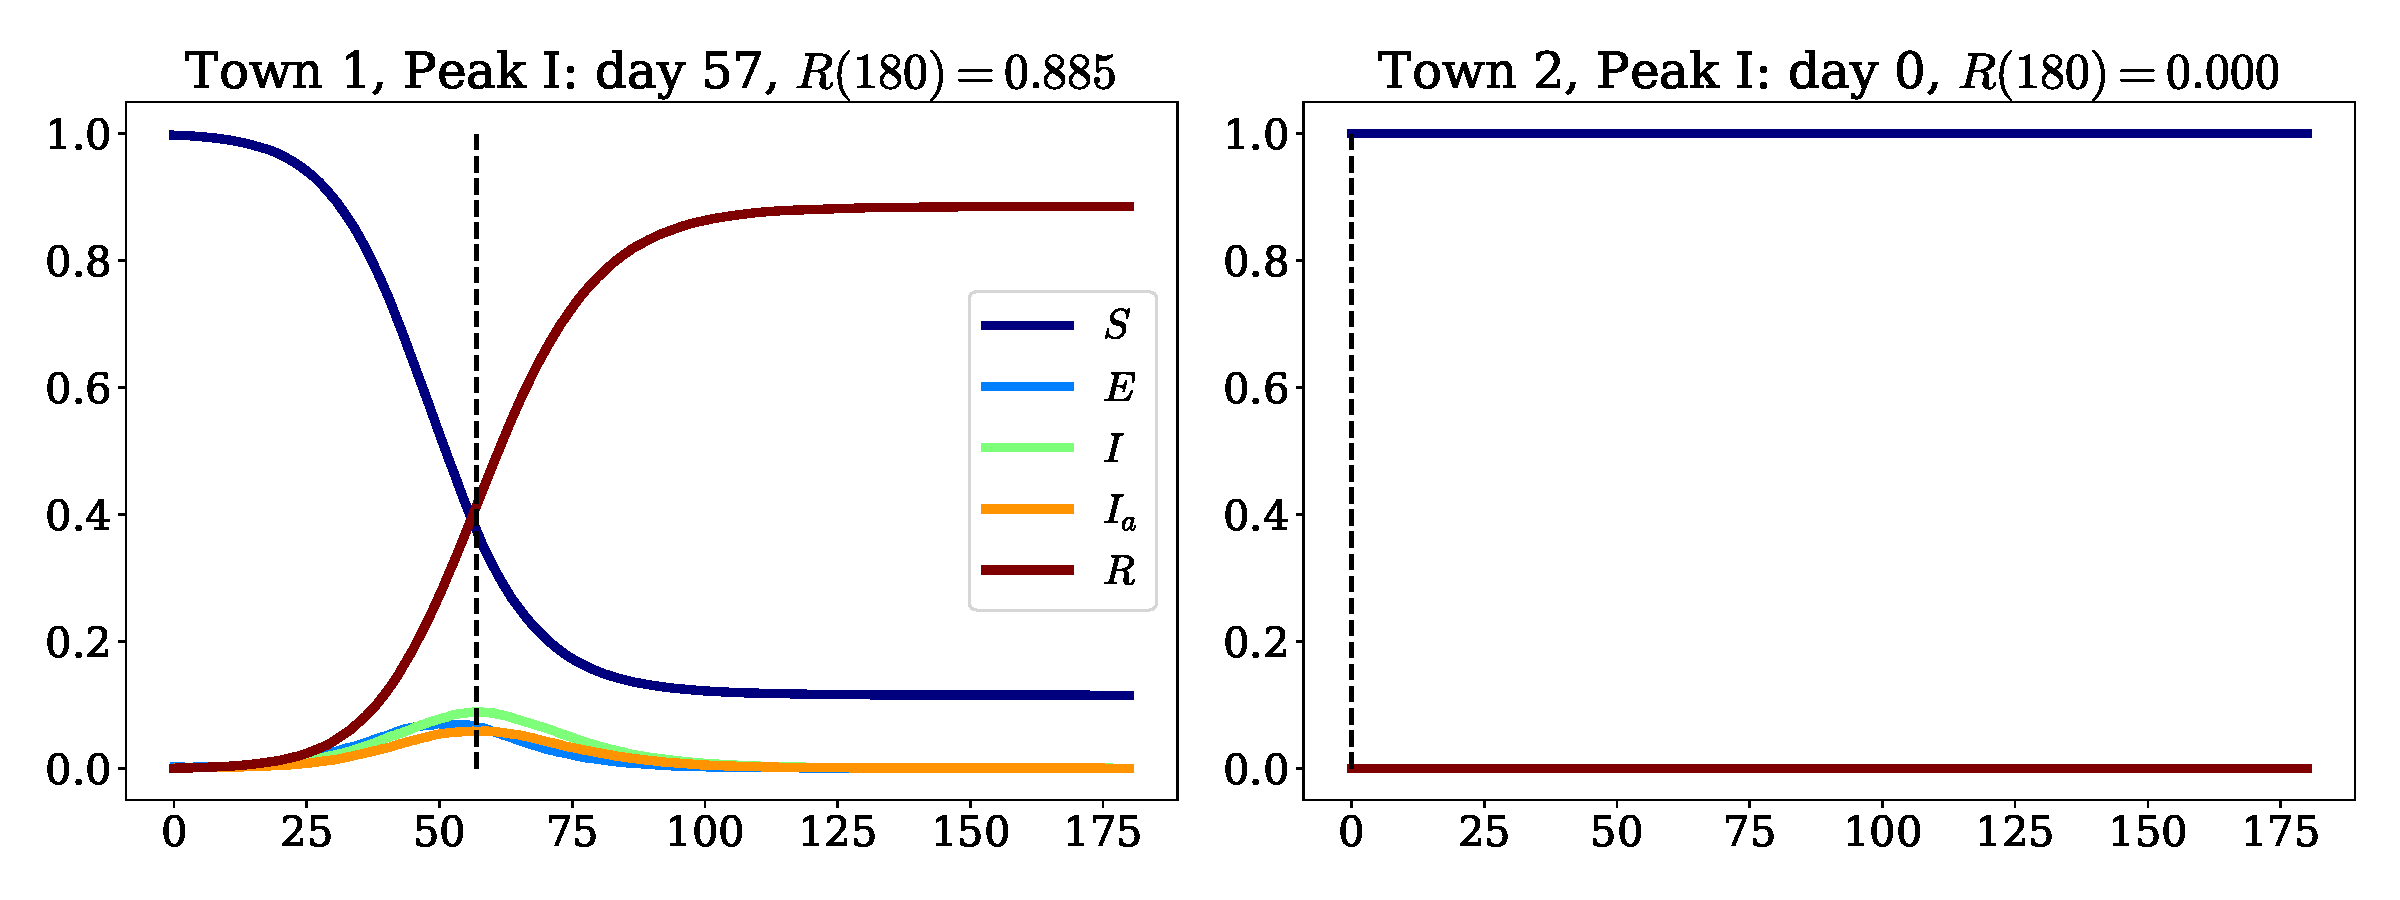
\includegraphics[width=.7\textwidth]{../plots/2D/two_towns2.pdf}
        \caption{Two towns, where everyone commutes, and the inital infection is only present in one of them. The plots shows that the infection is contained, as expected. Values are an average of 10 runs.}
        \label{All commuters}
    \end{figure}

    \begin{figure}[H]
        \centering
        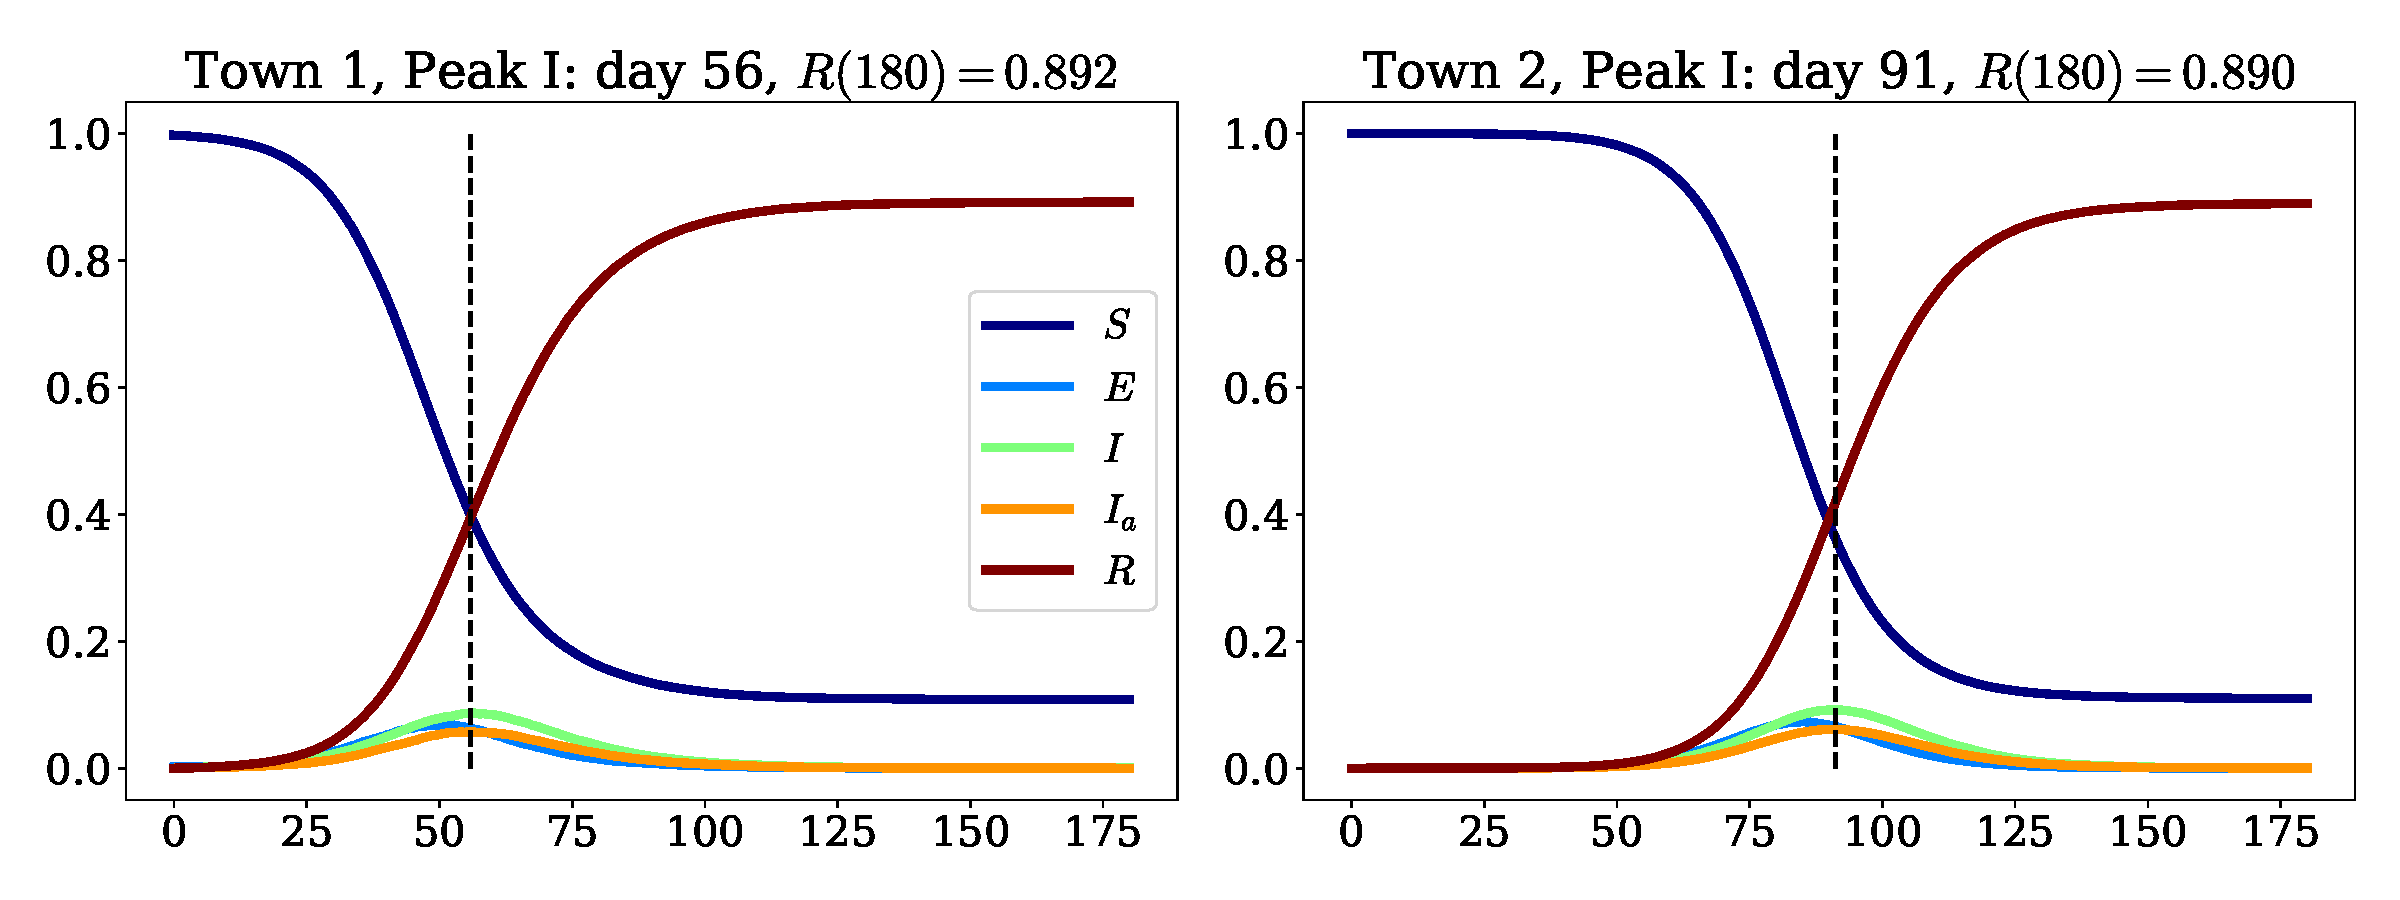
\includegraphics[width=.7\textwidth]{../plots/2D/two_towns.pdf}
        \caption{Spread of the infections in two connected towns. The lines are averages of 10 runs.}
        \label{two towns}
    \end{figure}

    \begin{figure}[H]
        \centering
        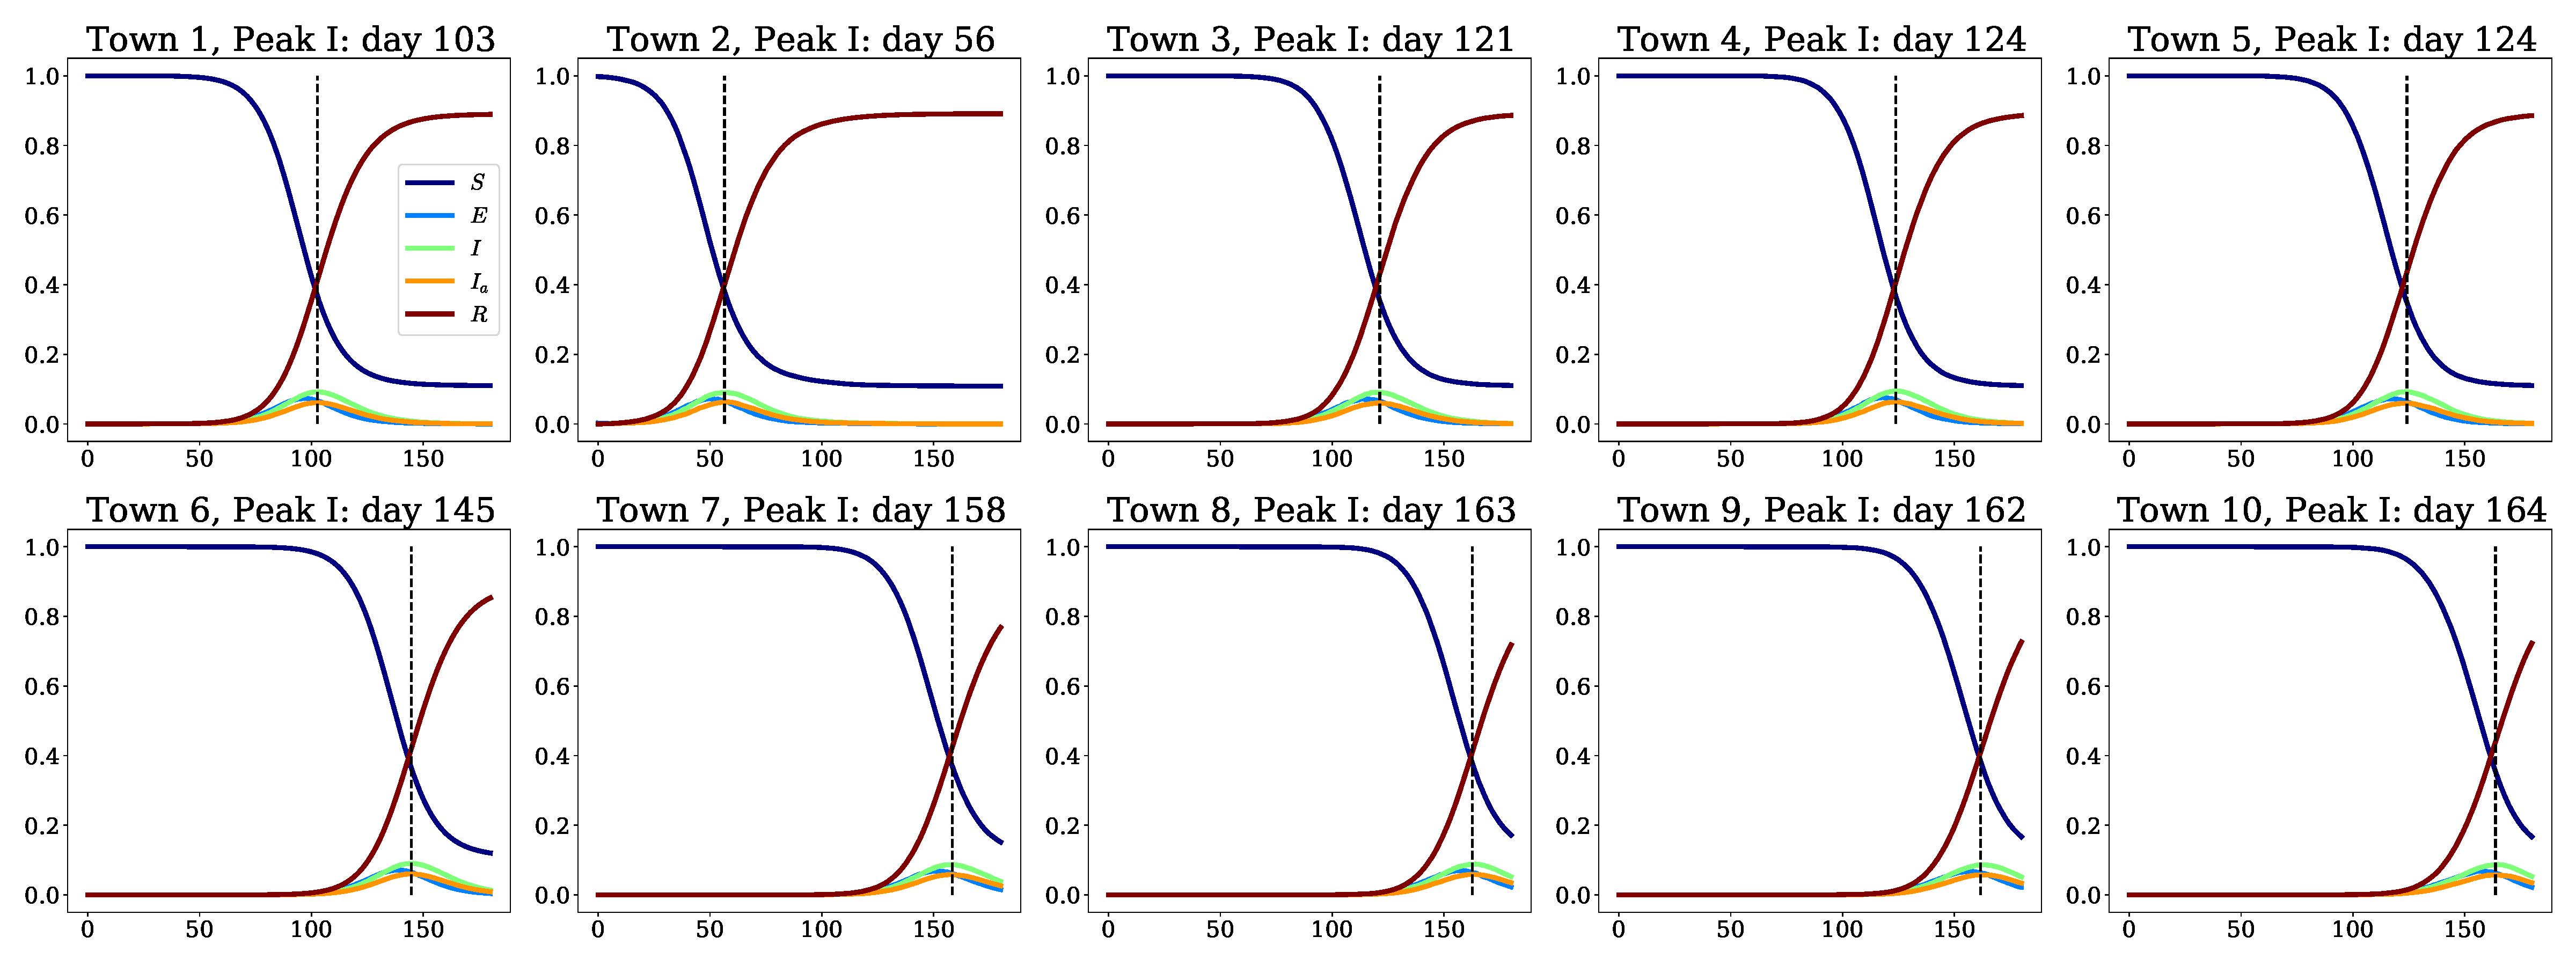
\includegraphics[width=\textwidth]{../plots/2D/nine_towns.pdf}
        \caption{The evloution of the infection in 10 connected towns. Lines are an average of 10 runs}
        \label{nine towns}
    \end{figure}

    The last system to be simulated is a model of Norway, with the working populace is spread throughout 356 cities and towns. 
    The simulation will be used to investigate the effects of reducing travel.
    This is done by cutting the off diagonal elements of the population matrix---representing those who travel to a different town for work---by 90\%, and increasing the population in their corresponding home town to keep the population living in that city constant.
    \autoref{pop structure} illustrates the population matrix before and after the lockdown, as well as the population distribution of towns and cities in question.
    The effect to be investigated is how lockdown changes how many towns have an outbreak at once.
    An outbreak is defined as more than a total of 10 people infected, where we count both symptomatic and and asymptomatic infections i.e. $I_\mathrm{tot}=I + I_a$.
    The simulation is run by starting with $E=50$ in town 1, Oslo, then taking the average of 10 runs for both population matrices.
    \autoref{towns infected} shows the evolution of the infection, in both cases. 
    On the left is the case without any restriction, and on the right is the case where commuting is reduced by 90\%. 
    This shows that the lockdown somewhat slows the spread.
    In the case of no lockdown, there is a period where all towns have a active infection, while the slows the spread down, resulting in a lower peak.
    \autoref{Oslo Bergen} compares the spread in the largest and second largest city, with and without lockdown.
    The largest town, town 1, is more or less unaffected, as it is where the spread started.
    The second largest town however, town 237, is affected.
    The peak in this town is delayed by around a month due to the lockdown.
    The total number of infections does not seem to be affected.

    \begin{figure}[H]
        \centering
        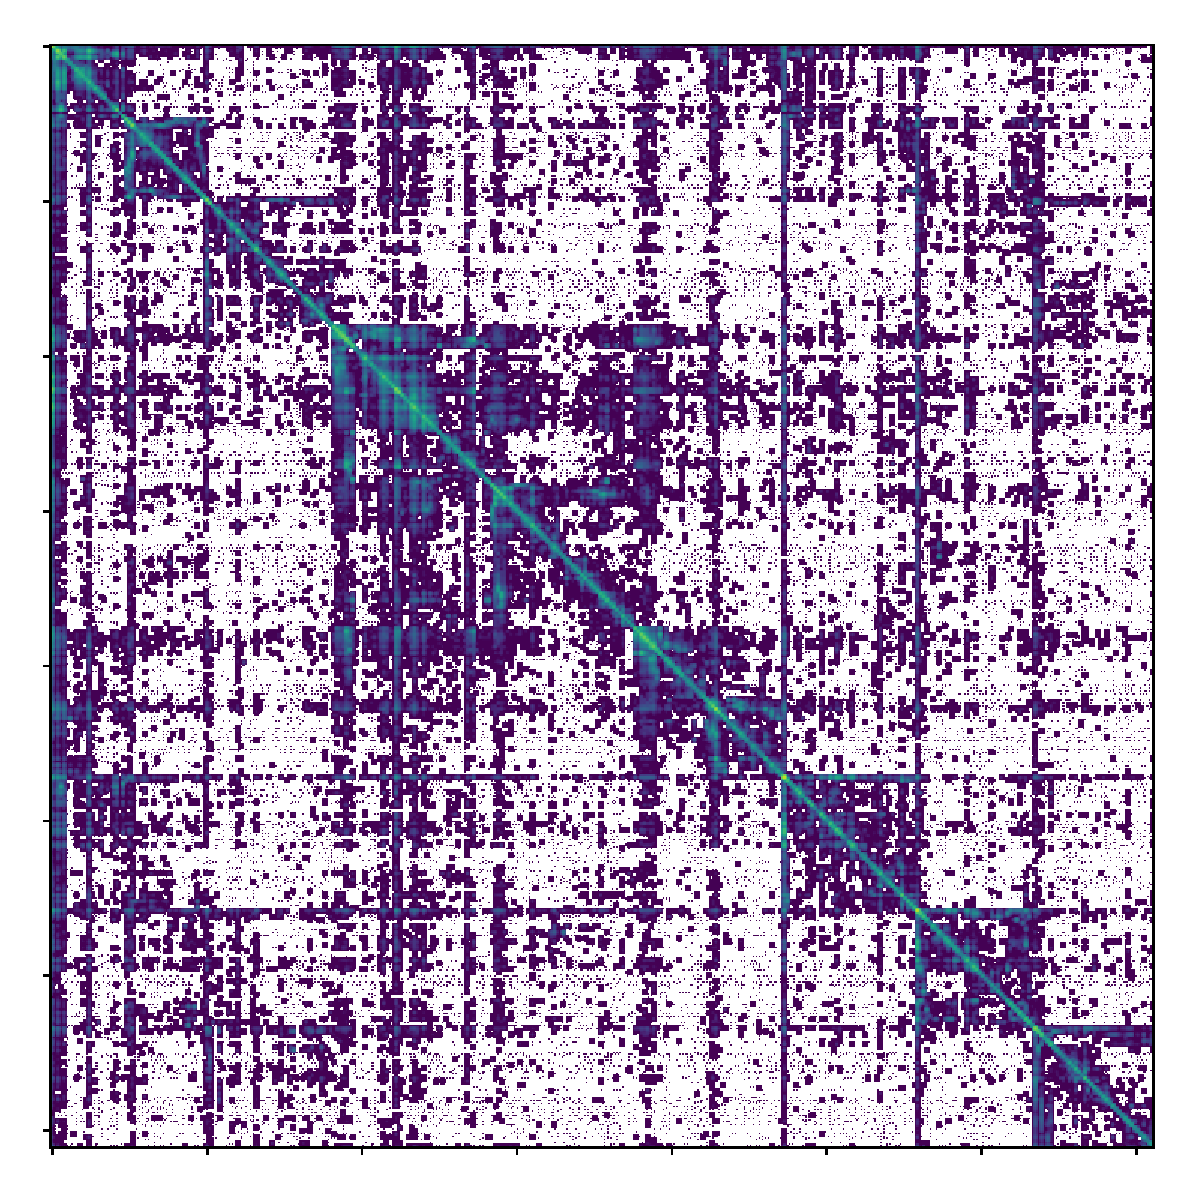
\includegraphics[width=.23\textwidth]{../plots/2D/pop_struct.pdf}
        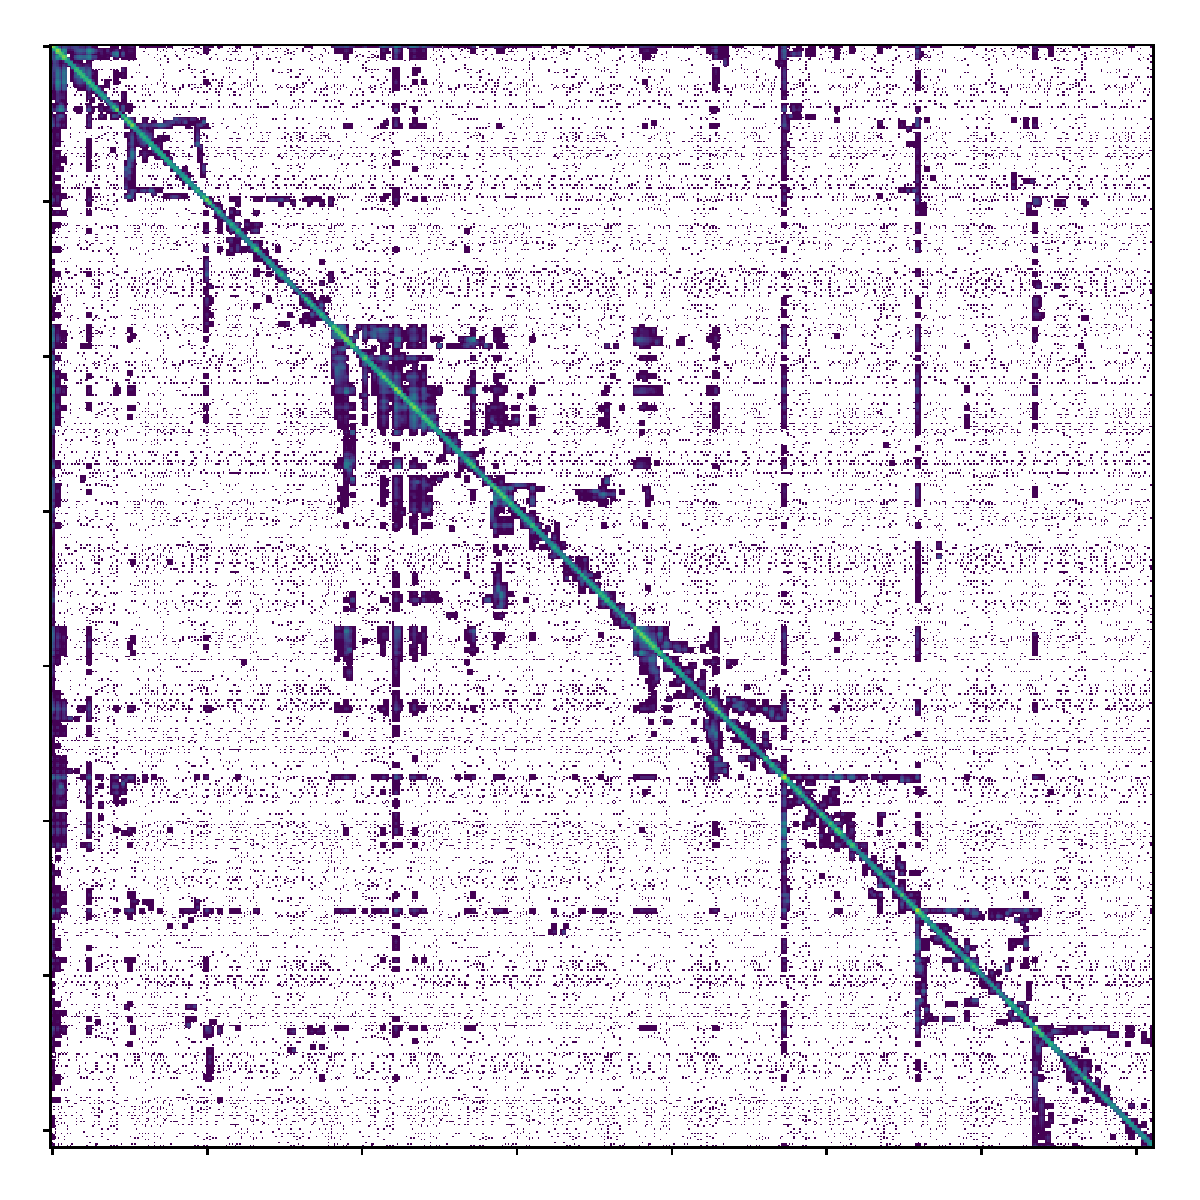
\includegraphics[width=.23\textwidth]{../plots/2D/pop_struct_lockdown.pdf}
        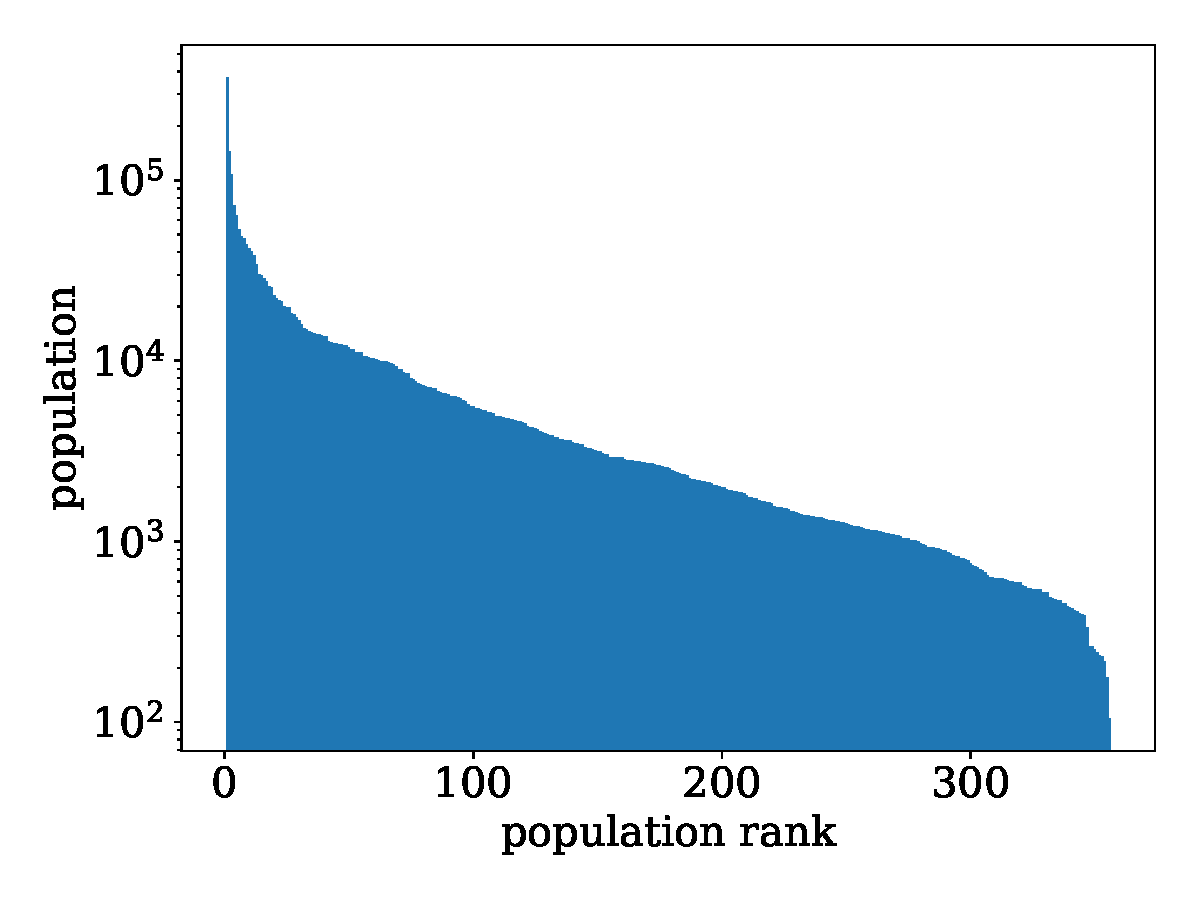
\includegraphics[width=.32\textwidth]{../plots/2D/pops.pdf}
        \caption{On the left, the Matrixed representing the popluation distribution in Norway, befor and after lockdown. On the right, sizes of the towns as afunction of the rank.}
        \label{pop structure}
    \end{figure}

    \begin{figure}[H]
        \centering
        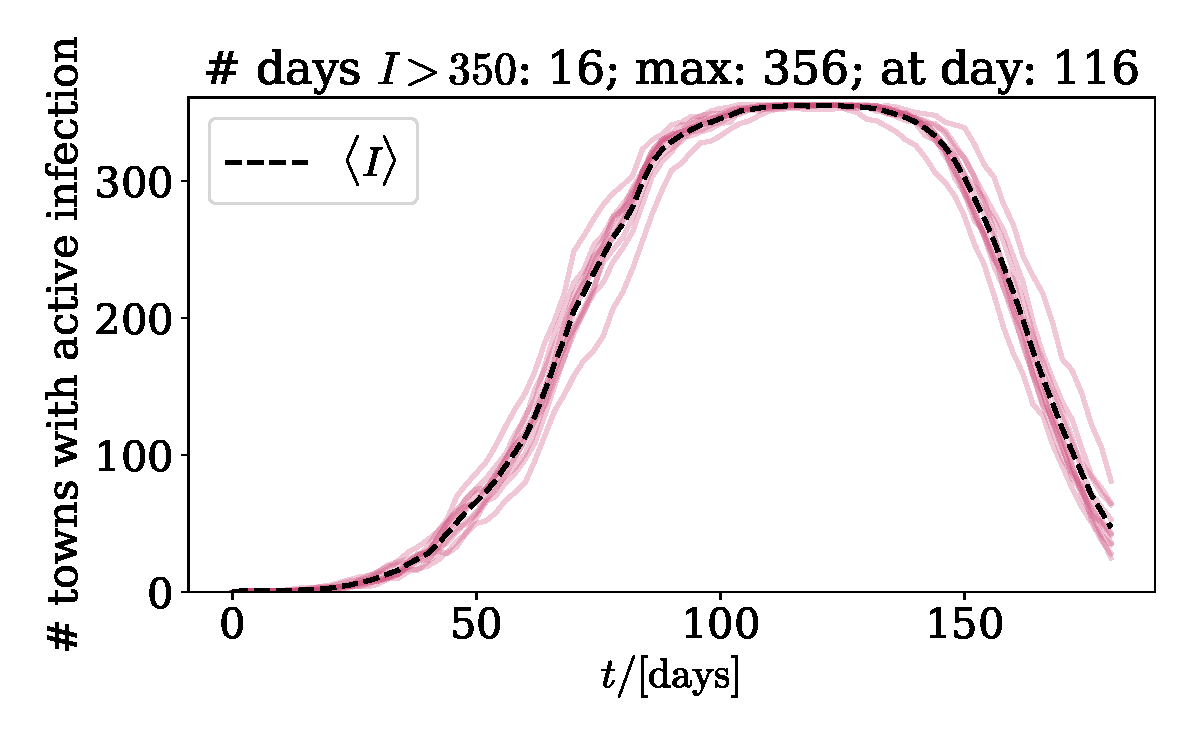
\includegraphics[width=.45\textwidth]{../plots/2D/num_infected.pdf}
        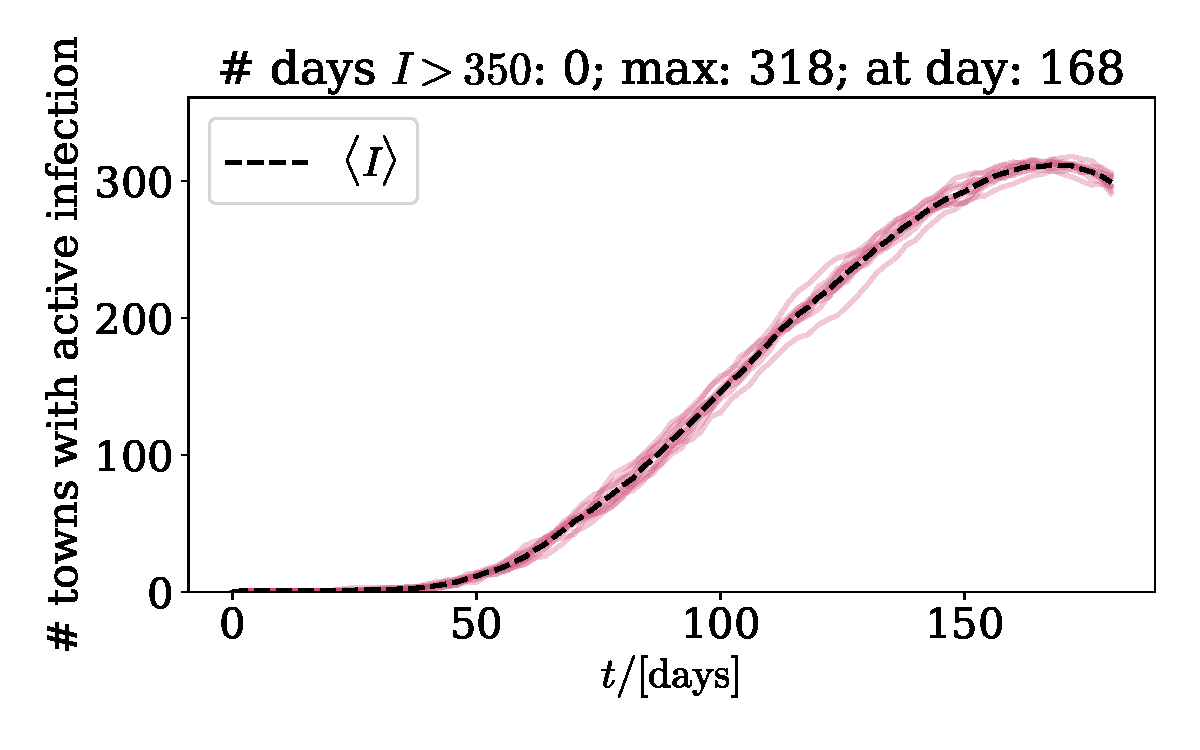
\includegraphics[width=.45\textwidth]{../plots/2D/num_infectedlockdown.pdf}
        \caption{The total number of towns with more than 10 infected. 
        The red, faded lines are a single simulation, while the dashed line is the average. 
        The plot to the right is the original populations, the plot on the right is after lockdown.}
        \label{towns infected}
    \end{figure}

    \begin{figure}[H]
        \centering
        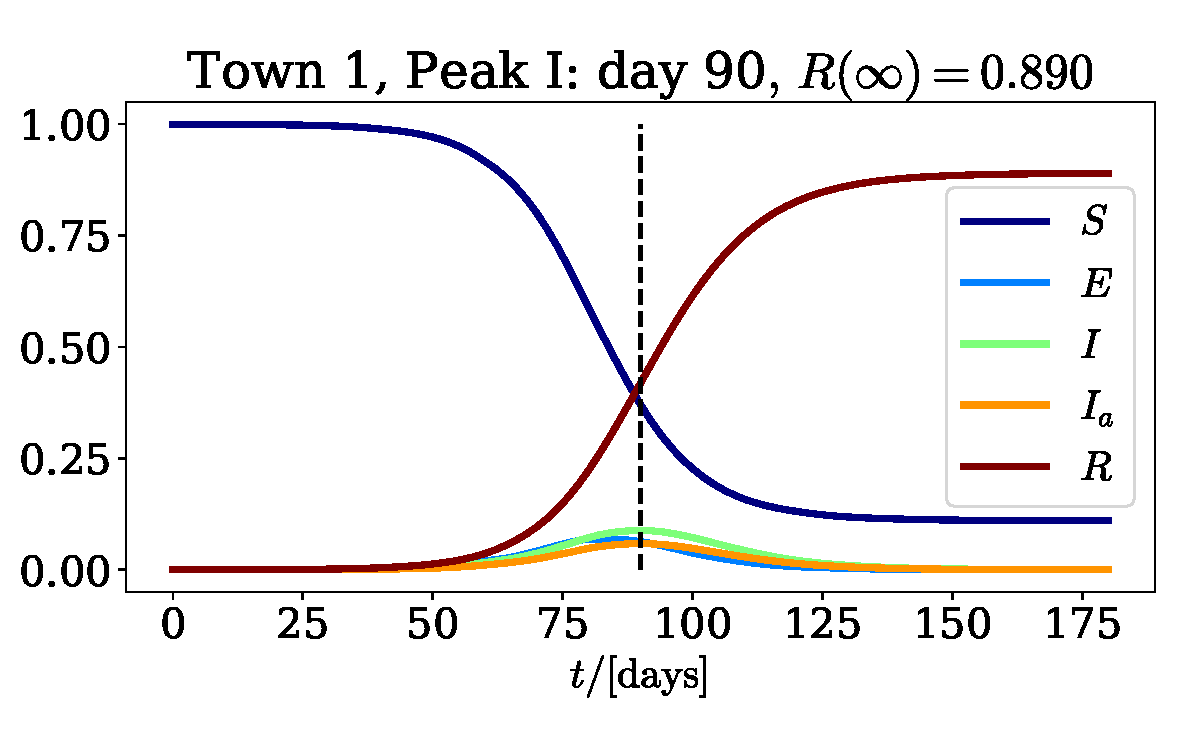
\includegraphics[width=.4\textwidth]{../plots/2D/Oslo.pdf}
        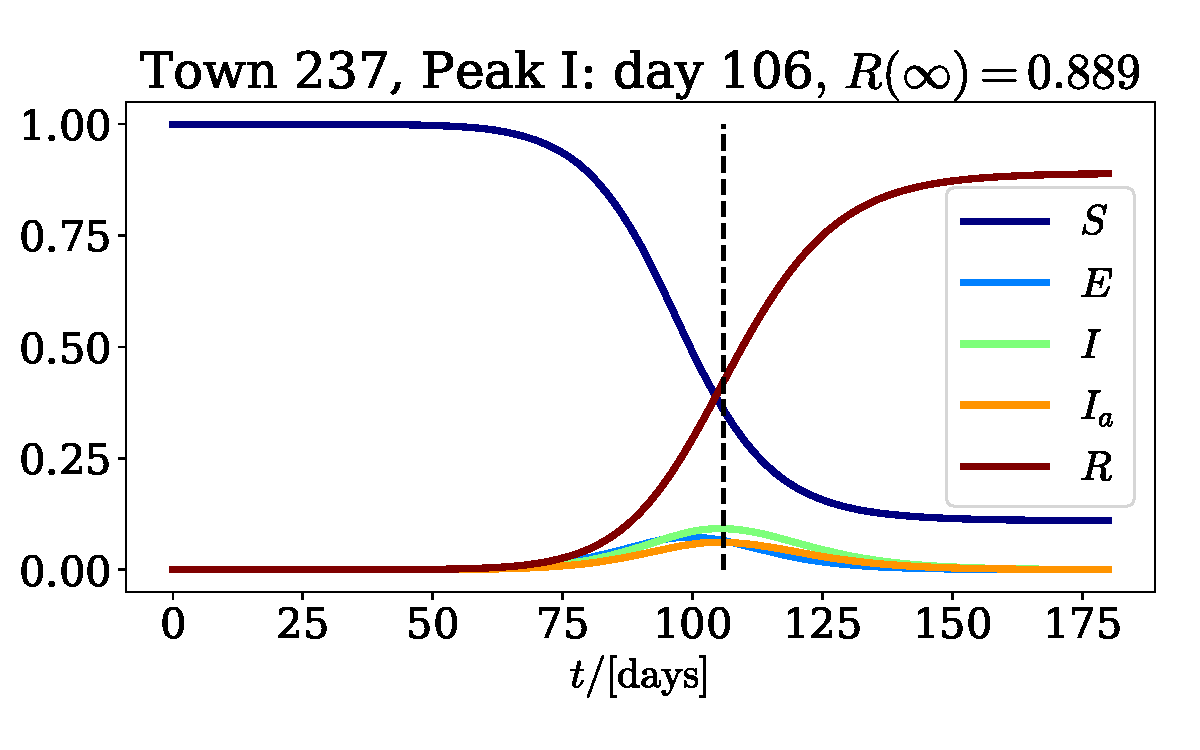
\includegraphics[width=.4\textwidth]{../plots/2D/Bergen.pdf}
        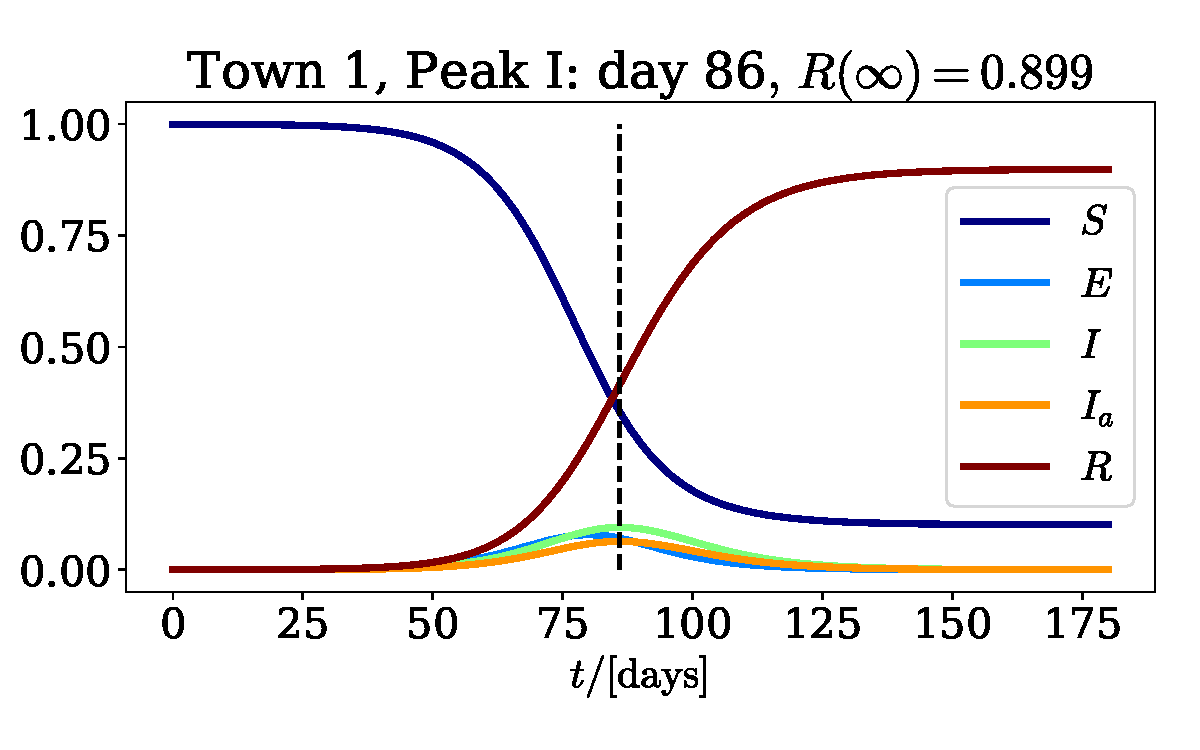
\includegraphics[width=.4\textwidth]{../plots/2D/Oslolockdown.pdf}
        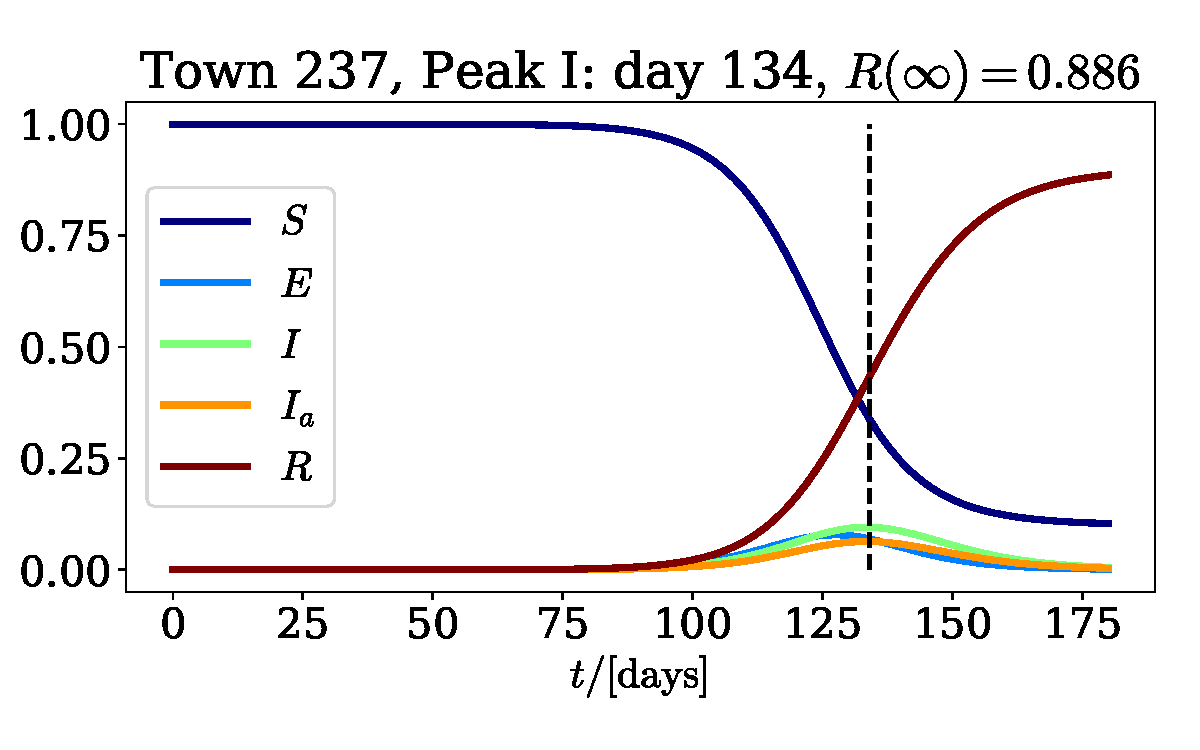
\includegraphics[width=.4\textwidth]{../plots/2D/Bergenlockdown.pdf}
        \caption{The infection in the two largest cities befor (top) and after (bottom) the lockdown.}
        \label{Oslo Bergen}
    \end{figure}
    
    \subsection*{Conclusion}
    This paper has documented the implementation, testing and result of several theoretical models of the spread of infections.
    The deterministic and stochastic SIR model, as well as the SEIIaR model with and without commuting have been investigated.
    Each model have been tested and are shown to give reliable results.
    The deterministic SIR model showed that $\beta \leq 0.228$ ensures that the total fraction of infected stays below 20\%, while a 60\% or more vaccinated populace ensures that the infection never enters exponential growth.
    The stochastic SIR model showed the probability for a infection to die out, while the SEIIaR was used to investigate the effects of isolating when getting symptoms.
    The simulation showed that the highest value of $r_s$ that stops exponential growth on average was $r_s=0.42$, 
    while the lowest measured value that ensures the probability of exponential growth is less than 50\% is $r_s=0.43$. 
    The uncertainties in these results were discussed.
    Lastly, the SEIIaR commuter model was used to investigate how the movement of people affect the model.
    It showed how an infection travel from town to town, with a delay, and that a sharp reduction in travel will delay the spread. 
    The model of Norway with a 90\% reduction in commuting, the peak of the infection as defined in this papaer was hit 52 days later, and was lower than the model without reduction in travel.
    \printbibliography
\end{document}